\documentclass[12pt,letterpaperpaper,openany]{book}
\usepackage{lmodern}
\usepackage{amssymb,amsmath}
\usepackage{ifxetex,ifluatex}
\usepackage{fixltx2e} % provides \textsubscript
\ifnum 0\ifxetex 1\fi\ifluatex 1\fi=0 % if pdftex
  \usepackage[T1]{fontenc}
  \usepackage[utf8]{inputenc}
\else % if luatex or xelatex
  \ifxetex
    \usepackage{mathspec}
  \else
    \usepackage{fontspec}
  \fi
  \defaultfontfeatures{Ligatures=TeX,Scale=MatchLowercase}
    \setmainfont[]{Charter}
    \setmonofont[Mapping=tex-ansi]{Source Code Pro}
\fi
% use upquote if available, for straight quotes in verbatim environments
\IfFileExists{upquote.sty}{\usepackage{upquote}}{}
% use microtype if available
\IfFileExists{microtype.sty}{%
\usepackage{microtype}
\UseMicrotypeSet[protrusion]{basicmath} % disable protrusion for tt fonts
}{}
\usepackage[margin=0.75in, letterpaper]{geometry}
\usepackage{hyperref}
\PassOptionsToPackage{usenames,dvipsnames}{color} % color is loaded by hyperref
\hypersetup{unicode=true,
            pdfauthor={Abhijit Dasgupta, PhD},
            colorlinks=true,
            linkcolor=Maroon,
            citecolor=Blue,
            urlcolor=Blue,
            breaklinks=true}
\urlstyle{same}  % don't use monospace font for urls
\usepackage{natbib}
\bibliographystyle{plainnat}
\usepackage{color}
\usepackage{fancyvrb}
\newcommand{\VerbBar}{|}
\newcommand{\VERB}{\Verb[commandchars=\\\{\}]}
\DefineVerbatimEnvironment{Highlighting}{Verbatim}{commandchars=\\\{\}}
% Add ',fontsize=\small' for more characters per line
\usepackage{framed}
\definecolor{shadecolor}{RGB}{248,248,248}
\newenvironment{Shaded}{\begin{snugshade}}{\end{snugshade}}
\newcommand{\AlertTok}[1]{\textcolor[rgb]{0.94,0.16,0.16}{#1}}
\newcommand{\AnnotationTok}[1]{\textcolor[rgb]{0.56,0.35,0.01}{\textbf{\textit{#1}}}}
\newcommand{\AttributeTok}[1]{\textcolor[rgb]{0.77,0.63,0.00}{#1}}
\newcommand{\BaseNTok}[1]{\textcolor[rgb]{0.00,0.00,0.81}{#1}}
\newcommand{\BuiltInTok}[1]{#1}
\newcommand{\CharTok}[1]{\textcolor[rgb]{0.31,0.60,0.02}{#1}}
\newcommand{\CommentTok}[1]{\textcolor[rgb]{0.56,0.35,0.01}{\textit{#1}}}
\newcommand{\CommentVarTok}[1]{\textcolor[rgb]{0.56,0.35,0.01}{\textbf{\textit{#1}}}}
\newcommand{\ConstantTok}[1]{\textcolor[rgb]{0.00,0.00,0.00}{#1}}
\newcommand{\ControlFlowTok}[1]{\textcolor[rgb]{0.13,0.29,0.53}{\textbf{#1}}}
\newcommand{\DataTypeTok}[1]{\textcolor[rgb]{0.13,0.29,0.53}{#1}}
\newcommand{\DecValTok}[1]{\textcolor[rgb]{0.00,0.00,0.81}{#1}}
\newcommand{\DocumentationTok}[1]{\textcolor[rgb]{0.56,0.35,0.01}{\textbf{\textit{#1}}}}
\newcommand{\ErrorTok}[1]{\textcolor[rgb]{0.64,0.00,0.00}{\textbf{#1}}}
\newcommand{\ExtensionTok}[1]{#1}
\newcommand{\FloatTok}[1]{\textcolor[rgb]{0.00,0.00,0.81}{#1}}
\newcommand{\FunctionTok}[1]{\textcolor[rgb]{0.00,0.00,0.00}{#1}}
\newcommand{\ImportTok}[1]{#1}
\newcommand{\InformationTok}[1]{\textcolor[rgb]{0.56,0.35,0.01}{\textbf{\textit{#1}}}}
\newcommand{\KeywordTok}[1]{\textcolor[rgb]{0.13,0.29,0.53}{\textbf{#1}}}
\newcommand{\NormalTok}[1]{#1}
\newcommand{\OperatorTok}[1]{\textcolor[rgb]{0.81,0.36,0.00}{\textbf{#1}}}
\newcommand{\OtherTok}[1]{\textcolor[rgb]{0.56,0.35,0.01}{#1}}
\newcommand{\PreprocessorTok}[1]{\textcolor[rgb]{0.56,0.35,0.01}{\textit{#1}}}
\newcommand{\RegionMarkerTok}[1]{#1}
\newcommand{\SpecialCharTok}[1]{\textcolor[rgb]{0.00,0.00,0.00}{#1}}
\newcommand{\SpecialStringTok}[1]{\textcolor[rgb]{0.31,0.60,0.02}{#1}}
\newcommand{\StringTok}[1]{\textcolor[rgb]{0.31,0.60,0.02}{#1}}
\newcommand{\VariableTok}[1]{\textcolor[rgb]{0.00,0.00,0.00}{#1}}
\newcommand{\VerbatimStringTok}[1]{\textcolor[rgb]{0.31,0.60,0.02}{#1}}
\newcommand{\WarningTok}[1]{\textcolor[rgb]{0.56,0.35,0.01}{\textbf{\textit{#1}}}}
\usepackage{longtable,booktabs}
\usepackage{graphicx,grffile}
\makeatletter
\def\maxwidth{\ifdim\Gin@nat@width>\linewidth\linewidth\else\Gin@nat@width\fi}
\def\maxheight{\ifdim\Gin@nat@height>\textheight\textheight\else\Gin@nat@height\fi}
\makeatother
% Scale images if necessary, so that they will not overflow the page
% margins by default, and it is still possible to overwrite the defaults
% using explicit options in \includegraphics[width, height, ...]{}
\setkeys{Gin}{width=\maxwidth,height=\maxheight,keepaspectratio}
\IfFileExists{parskip.sty}{%
\usepackage{parskip}
}{% else
\setlength{\parindent}{0pt}
\setlength{\parskip}{6pt plus 2pt minus 1pt}
}
\setlength{\emergencystretch}{3em}  % prevent overfull lines
\providecommand{\tightlist}{%
  \setlength{\itemsep}{0pt}\setlength{\parskip}{0pt}}
\setcounter{secnumdepth}{5}
% Redefines (sub)paragraphs to behave more like sections
\ifx\paragraph\undefined\else
\let\oldparagraph\paragraph
\renewcommand{\paragraph}[1]{\oldparagraph{#1}\mbox{}}
\fi
\ifx\subparagraph\undefined\else
\let\oldsubparagraph\subparagraph
\renewcommand{\subparagraph}[1]{\oldsubparagraph{#1}\mbox{}}
\fi

%%% Use protect on footnotes to avoid problems with footnotes in titles
\let\rmarkdownfootnote\footnote%
\def\footnote{\protect\rmarkdownfootnote}

%%% Change title format to be more compact
\usepackage{titling}

% Create subtitle command for use in maketitle
\newcommand{\subtitle}[1]{
  \posttitle{
    \begin{center}\large#1\end{center}
    }
}

\setlength{\droptitle}{-2em}

  \title{PS 312: Programming with R\\
Course Notes}
    \pretitle{\vspace{\droptitle}\centering\huge}
  \posttitle{\par}
    \author{Abhijit Dasgupta, PhD}
    \preauthor{\centering\large\emph}
  \postauthor{\par}
      \predate{\centering\large\emph}
  \postdate{\par}
    \date{Last updated: March 24, 2019}


\begin{document}
\maketitle

\hypertarget{welcome}{%
\chapter*{Welcome}\label{welcome}}
\addcontentsline{toc}{chapter}{Welcome}

This course is an introduction to the statistical programming language
\href{http://www.r-project.org}{R} and various applications. We will cover the entire data analytics pipeline from data ingestion to data wrangling, summarizing, modeling, visualizing and reporting, all using tools found within the R ecosystem.

The version of these notes you are reading now was built on
2019-03-24.

\hypertarget{reproducibility}{%
\section*{Reproducibility}\label{reproducibility}}
\addcontentsline{toc}{section}{Reproducibility}

These notes are written with \href{https://bookdown.org}{\texttt{bookdown}}, a R package for writing books using \href{https://rmarkdown.rstudio.com}{\texttt{rmarkdown}}.
All code in these notes were developed on R version 3.5.0 (2018-04-23), using
the same packages pre-installed in your virtual machines. When you're on your
own, you will need to install a recent version of R, and also install the
corresponding packages, on your computer, for all the code to work. A listing of
all the packages used in this course will be available as an appendix.

To build these notes locally, clone or \href{https://github.com/araastat/FSI_Book/archive/master.zip}{download} the
\href{https://github.com/araastat/FSI_Book}{Github repo} hosting these notes, unzip it if necessary, and double-click on \texttt{FSI\_Book.Rproj}. Assuming you have RStudio installed, this will open this project (more on \emph{RStudio Projects} later). You can then go to the console and enter the following code:

\begin{Shaded}
\begin{Highlighting}[]
\NormalTok{bookdown}\OperatorTok{::}\KeywordTok{render_book}\NormalTok{(}\StringTok{"index.Rmd"}\NormalTok{) }\CommentTok{# to build these notes}
\KeywordTok{browseURL}\NormalTok{(}\StringTok{"_book/index.html"}\NormalTok{) }\CommentTok{# to view it}
\end{Highlighting}
\end{Shaded}

\hypertarget{part-day-one-starting-up}{%
\part*{Day One: Starting Up}\label{part-day-one-starting-up}}
\addcontentsline{toc}{part}{Day One: Starting Up}

\hypertarget{what-is-r}{%
\chapter{What is R?}\label{what-is-r}}

\href{https://www.r-project.org}{R} is the
most popular\footnote{\url{https://spectrum.ieee.org/static/interactive-the-top-programming-languages-2018}} open source \emph{statistical programming language} in the world. It
allows you to

\begin{enumerate}
\def\labelenumi{\arabic{enumi}.}
\tightlist
\item
  read datasets written in a wide variety of formats,
\item
  clean and process the data,
\item
  derive summaries,
\item
  run analytics,
\item
  visualize
\item
  create automated reports, presentations, websites, dashboards and interactive applications
\end{enumerate}

R is not just a language, but an ecosystem comprising over 15,000 user- and corporation-developed
\emph{packages} or modules, all written in the R language for a variety of purposes. It is a very flexible and customizable language, which is why it is used by an estimated 2 million users worldwide for data analytics.
The question R users often ask is not ``Can it be done?'' but rather ``How can it be done?''. R is used
in areas as varied as healthcare, economics, forestry, oceanography, pharmaceuticals, artificial
intelligence and natural language processing.

Why is R so widely used? Some reasons are:

\begin{itemize}
\tightlist
\item
  R is open source, so it is accessible to anyone with a computer
\item
  Since the code in R and all its packages are open, the community of users can help debug it
  and make it more reliable and robust
\item
  The R ecosystem is very rich in tools for doing data analytics in particular, so there is almost
  certainly something available for almost any task
\item
  The community of R users worldwide is a very strong, well-connected group who are welcoming,
  ready to help, cooperative and inclusive. Many users find this community to be one of the most
  attractive things about R
\item
  R produces really nice customizable visualizations with relatively little effort, which was one of the
  first reasons for popularity.
\end{itemize}

\hypertarget{a-note-on-coding-and-programming}{%
\section*{A note on coding and programming}\label{a-note-on-coding-and-programming}}
\addcontentsline{toc}{section}{A note on coding and programming}

R does not have a \emph{point-and-click} interface that you are probably more familiar with
from Excel, Word or other computer applications. It requires you to \emph{code}, i.e.~write
instructions for the computer to, in the case of R, read, analyze, graph and report on datasets.

R is first and foremost a \textbf{language}. So, instead of thinking that this is some
geeky thing that ``programmers'' and ``IT people'' do, think of it as learning a language.
You will see that, like any language, it has nouns, verbs, adjectives and adverbs,
and you can create ``sentences'' that start with data and end in something useful like a
table, graph or document. With a traditional spoken and written language like French, Arabic, Farsi or Japanese, you learn it to
be able to interact with people at different posts around the world. With a programming language
like R, you will be able to interact with \textbf{data}, to make sense of it, to describe it,
and to present it.

\hypertarget{coding}{%
\subsection*{Coding}\label{coding}}
\addcontentsline{toc}{subsection}{Coding}

Coding is writing explicit instructions to a very literal, and in some ways, stupid machine.
The machine takes our code literally, and will do \textbf{exactly} what you tell it to do in the code. If
you are getting unexpected results, it's almost certainly your code that needs to be checked, not
the machine.

\hypertarget{r-the-language}{%
\subsection*{R, the language}\label{r-the-language}}
\addcontentsline{toc}{subsection}{R, the language}

As we will see, R has many elements of a language.

\begin{itemize}
\tightlist
\item
  \textbf{Objects}: These are the \emph{nouns}. We will act on objects to create new objects. Each object has a \emph{name} which we will treat as the nouns in our code.
\item
  \textbf{Functions}: These are the \emph{verbs}. Functions will act on objects to create new objects.
\item
  \textbf{The \texttt{\%\textgreater{}\%} operator}: This acts like the conjunction ``then'' to create ``sentences'' called \emph{pipes} or \emph{chains}.
\item
  \textbf{Optional function arguments}: These are adverbs which modify the action of the function (verb).
\end{itemize}

While writing code in R, we should be aware that R is \textbf{case-sensitive}, so \texttt{mydata} is a different object
than \texttt{myData} which is also different from \texttt{Mydata} and \texttt{My\_Data} and \texttt{MyData} and \texttt{my\_data}, and \texttt{mean}, which is a function in R, is different from \texttt{Mean} which is not defined in R.

\begin{quote}
You have to name all the objects you create in R if you want to see them again. Try and pick a
naming system that is simple yet descriptive, rather than \texttt{data1}. Two typical conventions that are used
are CamelCase and pothole\_case. So you could name a dataset of operational budgets for January, 2019 as
\texttt{operations\_budget\_2019\_jan} or \texttt{OperationsBudget2019Jan} or really anything you want, as long as it's
clear to you and doesn't include some forbidden characters like \texttt{-}, \texttt{@},\texttt{\$} which are reserved for
other purposes, or doesn't start with a number.

Some people have a system where data objects (which are called \texttt{data.frame} or \texttt{tibble} or \texttt{vector} or \texttt{matrix}) should be
capitalized, while function names should not. Data objects should probably be nouns and functions verbs, since that reminds us of their functions. There are different opinions. Some influential ones are
\href{http://adv-r.had.co.nz/Style.html}{here} and \href{https://google.github.io/styleguide/Rguide.xml}{here}. As they say, finding a good name is hard, but often worth the effort.
\end{quote}

The ultimate goal for every script file is to create a ``story'' using the language of R,
starting from data to create descriptions, understand patterns through visualization and modeling,
and analyzing the data in general. Scripts make this story reproducible, and also transferable to different data sets.

Of course, as with any beginner writer, your coding will be sloppy at first, will suffer many
stops and starts and strike-throughs and modifications and throwing things into the proverbial trash. With practice, this will become easier and smoother and more effective and more expressive. This workshop is designed to give you an initial push towards that goal.

So, let's start this journey.

\hypertarget{a-short-introduction-to-r-objects}{%
\section{A short introduction to R objects}\label{a-short-introduction-to-r-objects}}

\hypertarget{objects}{%
\subsection{Objects}\label{objects}}

The broad categorization of R objects in my mind are functions (verbs) and data objects (nouns).
Data objects are in turn of different types:

\begin{itemize}
\tightlist
\item
  \texttt{data.frame} or \texttt{tibble}: These are rectangular data sets much like you would see in a spreadsheet
\item
  \texttt{vector}: This is a 1-dimensional list of numbers or strings (words in the language sense), but all must be of the same kind (number or string)
\item
  \texttt{matrix}: This is a 2-dimensional list of numbers or strings, once again all of the same type
\item
  A single number or word
\item
  \texttt{list}: This is a catch-all bucket. Each element of a list can be literally any valid R object. So they could be \texttt{tibble}'s, or functions, or matrices, and different elements can be of different types.
\end{itemize}

Most objects we'll use in this workshop are going to be \texttt{data.frame} or \texttt{tibble} objects. (In case you're wondering, they're basically the same thing, but \texttt{tibble}'s have some modest additional functionality). R comes with a bunch of built-in datasets stored as \texttt{data.frame}s.

\begin{Shaded}
\begin{Highlighting}[]
\NormalTok{mtcars}
\end{Highlighting}
\end{Shaded}

\begin{verbatim}
##                      mpg cyl  disp  hp drat    wt  qsec vs am gear carb
## Mazda RX4           21.0   6 160.0 110 3.90 2.620 16.46  0  1    4    4
## Mazda RX4 Wag       21.0   6 160.0 110 3.90 2.875 17.02  0  1    4    4
## Datsun 710          22.8   4 108.0  93 3.85 2.320 18.61  1  1    4    1
## Hornet 4 Drive      21.4   6 258.0 110 3.08 3.215 19.44  1  0    3    1
## Hornet Sportabout   18.7   8 360.0 175 3.15 3.440 17.02  0  0    3    2
## Valiant             18.1   6 225.0 105 2.76 3.460 20.22  1  0    3    1
## Duster 360          14.3   8 360.0 245 3.21 3.570 15.84  0  0    3    4
## Merc 240D           24.4   4 146.7  62 3.69 3.190 20.00  1  0    4    2
## Merc 230            22.8   4 140.8  95 3.92 3.150 22.90  1  0    4    2
## Merc 280            19.2   6 167.6 123 3.92 3.440 18.30  1  0    4    4
## Merc 280C           17.8   6 167.6 123 3.92 3.440 18.90  1  0    4    4
## Merc 450SE          16.4   8 275.8 180 3.07 4.070 17.40  0  0    3    3
## Merc 450SL          17.3   8 275.8 180 3.07 3.730 17.60  0  0    3    3
## Merc 450SLC         15.2   8 275.8 180 3.07 3.780 18.00  0  0    3    3
## Cadillac Fleetwood  10.4   8 472.0 205 2.93 5.250 17.98  0  0    3    4
## Lincoln Continental 10.4   8 460.0 215 3.00 5.424 17.82  0  0    3    4
## Chrysler Imperial   14.7   8 440.0 230 3.23 5.345 17.42  0  0    3    4
## Fiat 128            32.4   4  78.7  66 4.08 2.200 19.47  1  1    4    1
## Honda Civic         30.4   4  75.7  52 4.93 1.615 18.52  1  1    4    2
## Toyota Corolla      33.9   4  71.1  65 4.22 1.835 19.90  1  1    4    1
## Toyota Corona       21.5   4 120.1  97 3.70 2.465 20.01  1  0    3    1
## Dodge Challenger    15.5   8 318.0 150 2.76 3.520 16.87  0  0    3    2
## AMC Javelin         15.2   8 304.0 150 3.15 3.435 17.30  0  0    3    2
## Camaro Z28          13.3   8 350.0 245 3.73 3.840 15.41  0  0    3    4
## Pontiac Firebird    19.2   8 400.0 175 3.08 3.845 17.05  0  0    3    2
## Fiat X1-9           27.3   4  79.0  66 4.08 1.935 18.90  1  1    4    1
## Porsche 914-2       26.0   4 120.3  91 4.43 2.140 16.70  0  1    5    2
## Lotus Europa        30.4   4  95.1 113 3.77 1.513 16.90  1  1    5    2
## Ford Pantera L      15.8   8 351.0 264 4.22 3.170 14.50  0  1    5    4
## Ferrari Dino        19.7   6 145.0 175 3.62 2.770 15.50  0  1    5    6
## Maserati Bora       15.0   8 301.0 335 3.54 3.570 14.60  0  1    5    8
## Volvo 142E          21.4   4 121.0 109 4.11 2.780 18.60  1  1    4    2
\end{verbatim}

A \texttt{data.frame} can be acted upon by different functions to help describe it and extract elements from it. For example, to see the size of the data, we use

\begin{Shaded}
\begin{Highlighting}[]
\KeywordTok{dim}\NormalTok{(mtcars)}
\end{Highlighting}
\end{Shaded}

\begin{verbatim}
## [1] 32 11
\end{verbatim}

Data sets often have row names and column names. These can be extracted by the functions \texttt{rownames} and
\texttt{colnames} or \texttt{names}:

\begin{Shaded}
\begin{Highlighting}[]
\KeywordTok{rownames}\NormalTok{(mtcars)}
\end{Highlighting}
\end{Shaded}

\begin{verbatim}
##  [1] "Mazda RX4"           "Mazda RX4 Wag"       "Datsun 710"         
##  [4] "Hornet 4 Drive"      "Hornet Sportabout"   "Valiant"            
##  [7] "Duster 360"          "Merc 240D"           "Merc 230"           
## [10] "Merc 280"            "Merc 280C"           "Merc 450SE"         
## [13] "Merc 450SL"          "Merc 450SLC"         "Cadillac Fleetwood" 
## [16] "Lincoln Continental" "Chrysler Imperial"   "Fiat 128"           
## [19] "Honda Civic"         "Toyota Corolla"      "Toyota Corona"      
## [22] "Dodge Challenger"    "AMC Javelin"         "Camaro Z28"         
## [25] "Pontiac Firebird"    "Fiat X1-9"           "Porsche 914-2"      
## [28] "Lotus Europa"        "Ford Pantera L"      "Ferrari Dino"       
## [31] "Maserati Bora"       "Volvo 142E"
\end{verbatim}

\begin{Shaded}
\begin{Highlighting}[]
\KeywordTok{names}\NormalTok{(mtcars)}
\end{Highlighting}
\end{Shaded}

\begin{verbatim}
##  [1] "mpg"  "cyl"  "disp" "hp"   "drat" "wt"   "qsec" "vs"   "am"   "gear"
## [11] "carb"
\end{verbatim}

Both of these are valid R objects that are vectors of strings. You could save them for future use by \emph{assigning} them a name using the assignment operator \texttt{\textless{}-}. So if you wanted to store the row names, which are the makes and models of the cars in this data set (this structure is not desirable, as we'll discuss later), you could run

\begin{Shaded}
\begin{Highlighting}[]
\NormalTok{car_names <-}\StringTok{ }\KeywordTok{rownames}\NormalTok{(mtcars)}
\end{Highlighting}
\end{Shaded}

You can see that this is stored in R for current use, either by typing \texttt{ls()} in the console (for ``list'') or by looking in the \texttt{Environment} pane in RStudio.

\begin{quote}
The output of any function is a valid R object, and so you can always store the results of the
function by assigning it a name, as above.
\end{quote}

\hypertarget{extracting-elements-from-objects}{%
\subsection{Extracting elements from objects}\label{extracting-elements-from-objects}}

We can see the structure of any object by using the function \texttt{str}.

\begin{Shaded}
\begin{Highlighting}[]
\KeywordTok{str}\NormalTok{(mtcars)}
\end{Highlighting}
\end{Shaded}

\begin{verbatim}
## 'data.frame':    32 obs. of  11 variables:
##  $ mpg : num  21 21 22.8 21.4 18.7 18.1 14.3 24.4 22.8 19.2 ...
##  $ cyl : num  6 6 4 6 8 6 8 4 4 6 ...
##  $ disp: num  160 160 108 258 360 ...
##  $ hp  : num  110 110 93 110 175 105 245 62 95 123 ...
##  $ drat: num  3.9 3.9 3.85 3.08 3.15 2.76 3.21 3.69 3.92 3.92 ...
##  $ wt  : num  2.62 2.88 2.32 3.21 3.44 ...
##  $ qsec: num  16.5 17 18.6 19.4 17 ...
##  $ vs  : num  0 0 1 1 0 1 0 1 1 1 ...
##  $ am  : num  1 1 1 0 0 0 0 0 0 0 ...
##  $ gear: num  4 4 4 3 3 3 3 4 4 4 ...
##  $ carb: num  4 4 1 1 2 1 4 2 2 4 ...
\end{verbatim}

This tells us that \texttt{mtcars} is a \texttt{data.frame} with 32 observations (rows) and 11 variables (columns).
Each variable has a name, and all the variables are numeric.

\begin{quote}
\texttt{data.frame} objects are like lists, in that each column can be of a different type. This is a very
powerful structure, since we can keep all sorts of data together, and can load spreadsheets with
diverse kinds of data easily into R
\end{quote}

To extract the \texttt{mpg} variable from this data set, there are a few equivalent methods. My preferred method is \texttt{mtcars{[},\textquotesingle{}mpg\textquotesingle{}{]}}, i.e., extract the \emph{column} named ``mpg'' from this data set. Notice that we're using \texttt{{[}{]}} while functions use \texttt{()}. This format of extraction will work when you're extracting more than one variable, as we'll see below. Other ways include \texttt{mtcars{[}{[}\textquotesingle{}mpg\textquotesingle{}{]}{]}} and \texttt{mtcars\$mpg}, which are
the \texttt{list} way and a \texttt{data.frame}-specific shortcut.

\begin{quote}
You can also extract elements by position, either using the \texttt{{[},{]}} or \texttt{{[}{[}{]}{]}} forms. So, to extract an
element in the 2nd row and 4th column, you'd have to use the matrix notation as \texttt{mtcars{[}2,4{]}}. To
extract the 4th column, you could use either \texttt{mtcars{[},4{]}} or \texttt{mtcars{[}{[}4{]}{]}}. To extract the 2nd row,
you'd again use the matrix notation as \texttt{mtcars{[}2,{]}}.
\end{quote}

If we want to extract the mpg, cyl and disp variables at once to create a new \texttt{data.frame}, you can
use either the matrix notation \texttt{mtcars{[},c(\textquotesingle{}mpg\textquotesingle{},\textquotesingle{}cyl\textquotesingle{},\textquotesingle{}disp\textquotesingle{}){]}} or the list notation \texttt{mtcars{[}{[}c(\textquotesingle{}mpg\textquotesingle{},\textquotesingle{}cyl\textquotesingle{},\textquotesingle{}disp\textquotesingle{}){]}{]}}. The \texttt{c()} function stands for \emph{concatenate} and is the function used to \textbf{create} vectors. We'll actually see a much more user-friendly way of doing this in the data munging section (Chapter \ref{sec:data-munging}).

\begin{quote}
\textbf{Advanced note:} A \texttt{data.frame} object is really a \texttt{list} object where all the elements are vectors
of the same length, and which happen to have names assigned to them. The object also looks like a matrix
or 2-dimensional array visually. So both notations were allowed to be valid for \texttt{data.frame} objects.
\end{quote}

\hypertarget{r-packages}{%
\section{R Packages}\label{r-packages}}

Packages are modules of R code that enhance the capabilities of R. Many packages are well established and curated, and have to go through a strict software compatibility review before allowed on \href{https://cran.rstudio.com}{CRAN}.

\hypertarget{installing-packages}{%
\subsection*{Installing packages}\label{installing-packages}}
\addcontentsline{toc}{subsection}{Installing packages}

Installing packages on your computer can be done from the RStudio menu (\texttt{Tools\ \textgreater{}\ Install\ Packages}),
or by running the command \texttt{install.packages(\textless{}package\ name\textgreater{},\ repos\ =\ "https://cran.rstudio.com")}. For example, to install the \texttt{readxl} package, which we will use shortly, we would run the code

\begin{Shaded}
\begin{Highlighting}[]
\KeywordTok{install.packages}\NormalTok{(}\StringTok{"readxl"}\NormalTok{, }\DataTypeTok{repos=}\StringTok{"https://cran.rstudio.com"}\NormalTok{)}
\end{Highlighting}
\end{Shaded}

\begin{quote}
You can set the default repository in RStudio, in \texttt{Tools\ \textgreater{}\ Global\ Options}.
\end{quote}

\begin{quote}
Be aware that everything here is case-sensitive
\end{quote}

Another way to install packages is to go to the \texttt{Packages} pane in RStudio, use the search bar there to
find the package you want to install, and then click the checkbox beside the name. This is convenient,
but not very reproducible if you have to move to a different computer, so it's generally discouraged.

How do you find packages? Glad you asked. The easiest way to find packages on CRAN is actually through the RStudio \texttt{Packages} pane, where the entire set of available packages are listed with a brief, top-line description. You can click on the package name to see a much more detailed overview of the packages, and many packages do have vignettes which give more information. However, once you've found the package you want, you should really code it up with \texttt{install.packages}, so that you can save the script for later when you might need to remember it again.

\hypertarget{loading-packages-in-r}{%
\subsection{Loading packages in R}\label{loading-packages-in-r}}

We will use several packages to enhance our experience and get going faster. However, to use a package, you must first load it into R. To load a package into R, you use the function \texttt{library} (ironically).

The first package we will load is the \texttt{tidyverse} package. This is actually a meta-package, which in turn loads a bunch of other packages. These form a core group of useful packages that are widely used, including

\begin{itemize}
\tightlist
\item
  readr (reading data from text files)
\item
  tidyr (Manipulation, pivoting)
\item
  dplyr (summarize, aggregate, filter)
\item
  ggplot2 (visualization)
\item
  purrr (functions applied across data structures, meta-programming)
\item
  stringr (string manipulation)
\item
  forcats (categorical data)
\end{itemize}

In addition, we'll load the \texttt{readxl} package for reading Excel files.

\begin{Shaded}
\begin{Highlighting}[]
\KeywordTok{library}\NormalTok{(tidyverse)}
\KeywordTok{library}\NormalTok{(readxl)}
\end{Highlighting}
\end{Shaded}

\hypertarget{r-resources}{%
\section{R Resources}\label{r-resources}}

There are many high quality resources for learning R available online. This is a selection of
what I find most useful.

\begin{enumerate}
\def\labelenumi{\arabic{enumi}.}
\tightlist
\item
  \href{https://cran.rstudio.com/web/views}{CRAN Task Views}: These are curated lists of R packages for various purposes, ranging from econometrics to mathematics, finance, imaging, social sciences, time series, spatial analyses and more.
\item
  \href{https://www.rstudio.com/resources/cheatsheets/}{RStudio Cheatsheets}: These are high-quality
  cheatsheets about different aspects of the R analytic pipeline.
\item
  \href{https://stackoverflow.com/questions/tagged/r}{StackOverflow \#r}: The \texttt{r} tag on StackOverflow is
  \emph{the} place to find answers about R
\item
  \href{https://twitter.com/hashtag/rstats}{Twitter \#rstats}: The who's who of R hang out at the \#rstats hashtag, and questions can get answered very quickly. Also a way to find out what new packages are coming up
\item
  \href{http://www.r-bloggers.com}{R-Bloggers}: A blog aggregator which collects a few hundred R-related blogs in one place (including mine, in the interests of disclosure)
\item
  \href{http://r-seek.org}{RSeek}: When one realizes that R is just a letter in the alphabet, Google searches can be a bit difficult. RSeek has created a custom search targeted at R-related topics, sites and packages on the web.
\end{enumerate}

\hypertarget{rstudio-your-development-environment-authoring-program}{%
\chapter{RStudio, your development environment (authoring program)}\label{rstudio-your-development-environment-authoring-program}}

While R is the language we will learn, \href{http://www.rstudio.com}{RStudio} is the interface
(or \emph{integrated development environment}) we will use to write it, interact with it, and see our
results. RStudio provides by far the most user-friendly interface to R (though it's not point-and-click).

This is the ``journal'' or ``notebook'' in which you will start your writing journey in R

\hypertarget{starting-rstudio}{%
\section*{Starting RStudio}\label{starting-rstudio}}
\addcontentsline{toc}{section}{Starting RStudio}

When you open RStudio, either from your desktop or from the Start menu, you'll
see something like this:

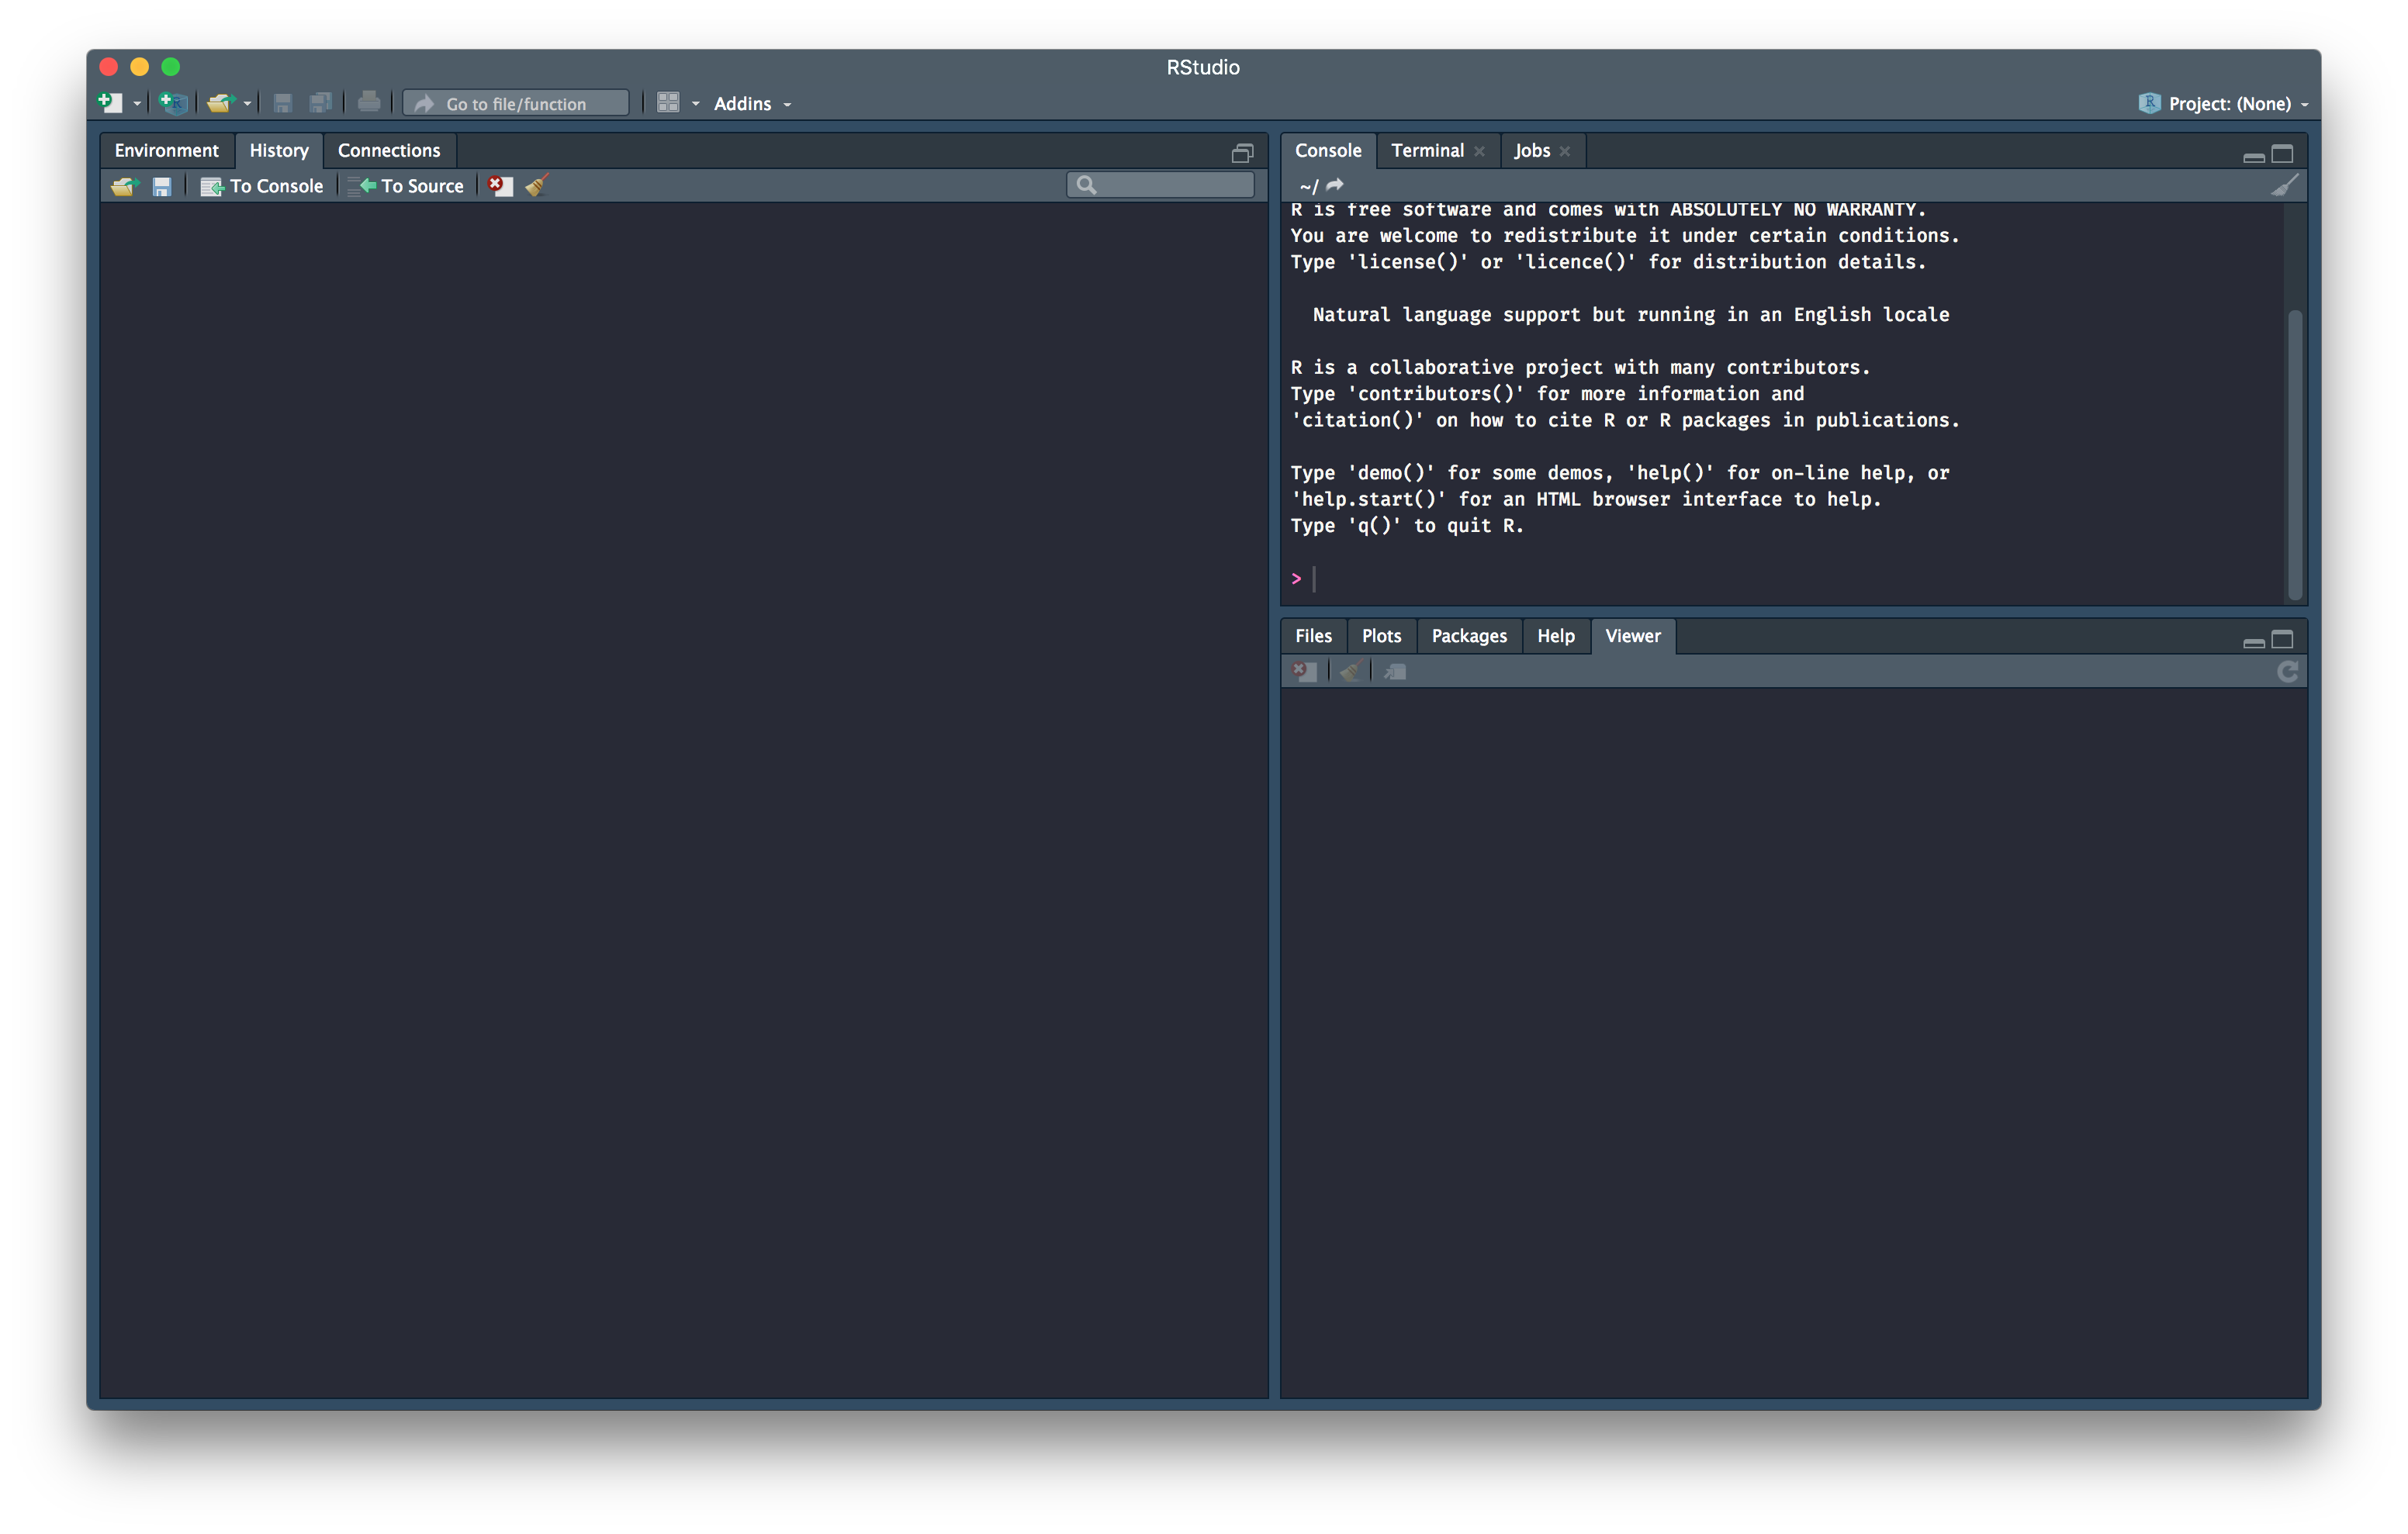
\includegraphics{img/RStudio.png}

\begin{quote}
I'll note that I've done some customization to my console, which you can also do by going to
\texttt{Tools\ \textgreater{}\ Global\ Options}. Your screen will most likely have a white rather than a dark background
\end{quote}

You can open a new panel for an R script using either \texttt{File\ \textgreater{}\ New\ File\ \textgreater{}\ R\ Script} or
using the button at the top left of the window:

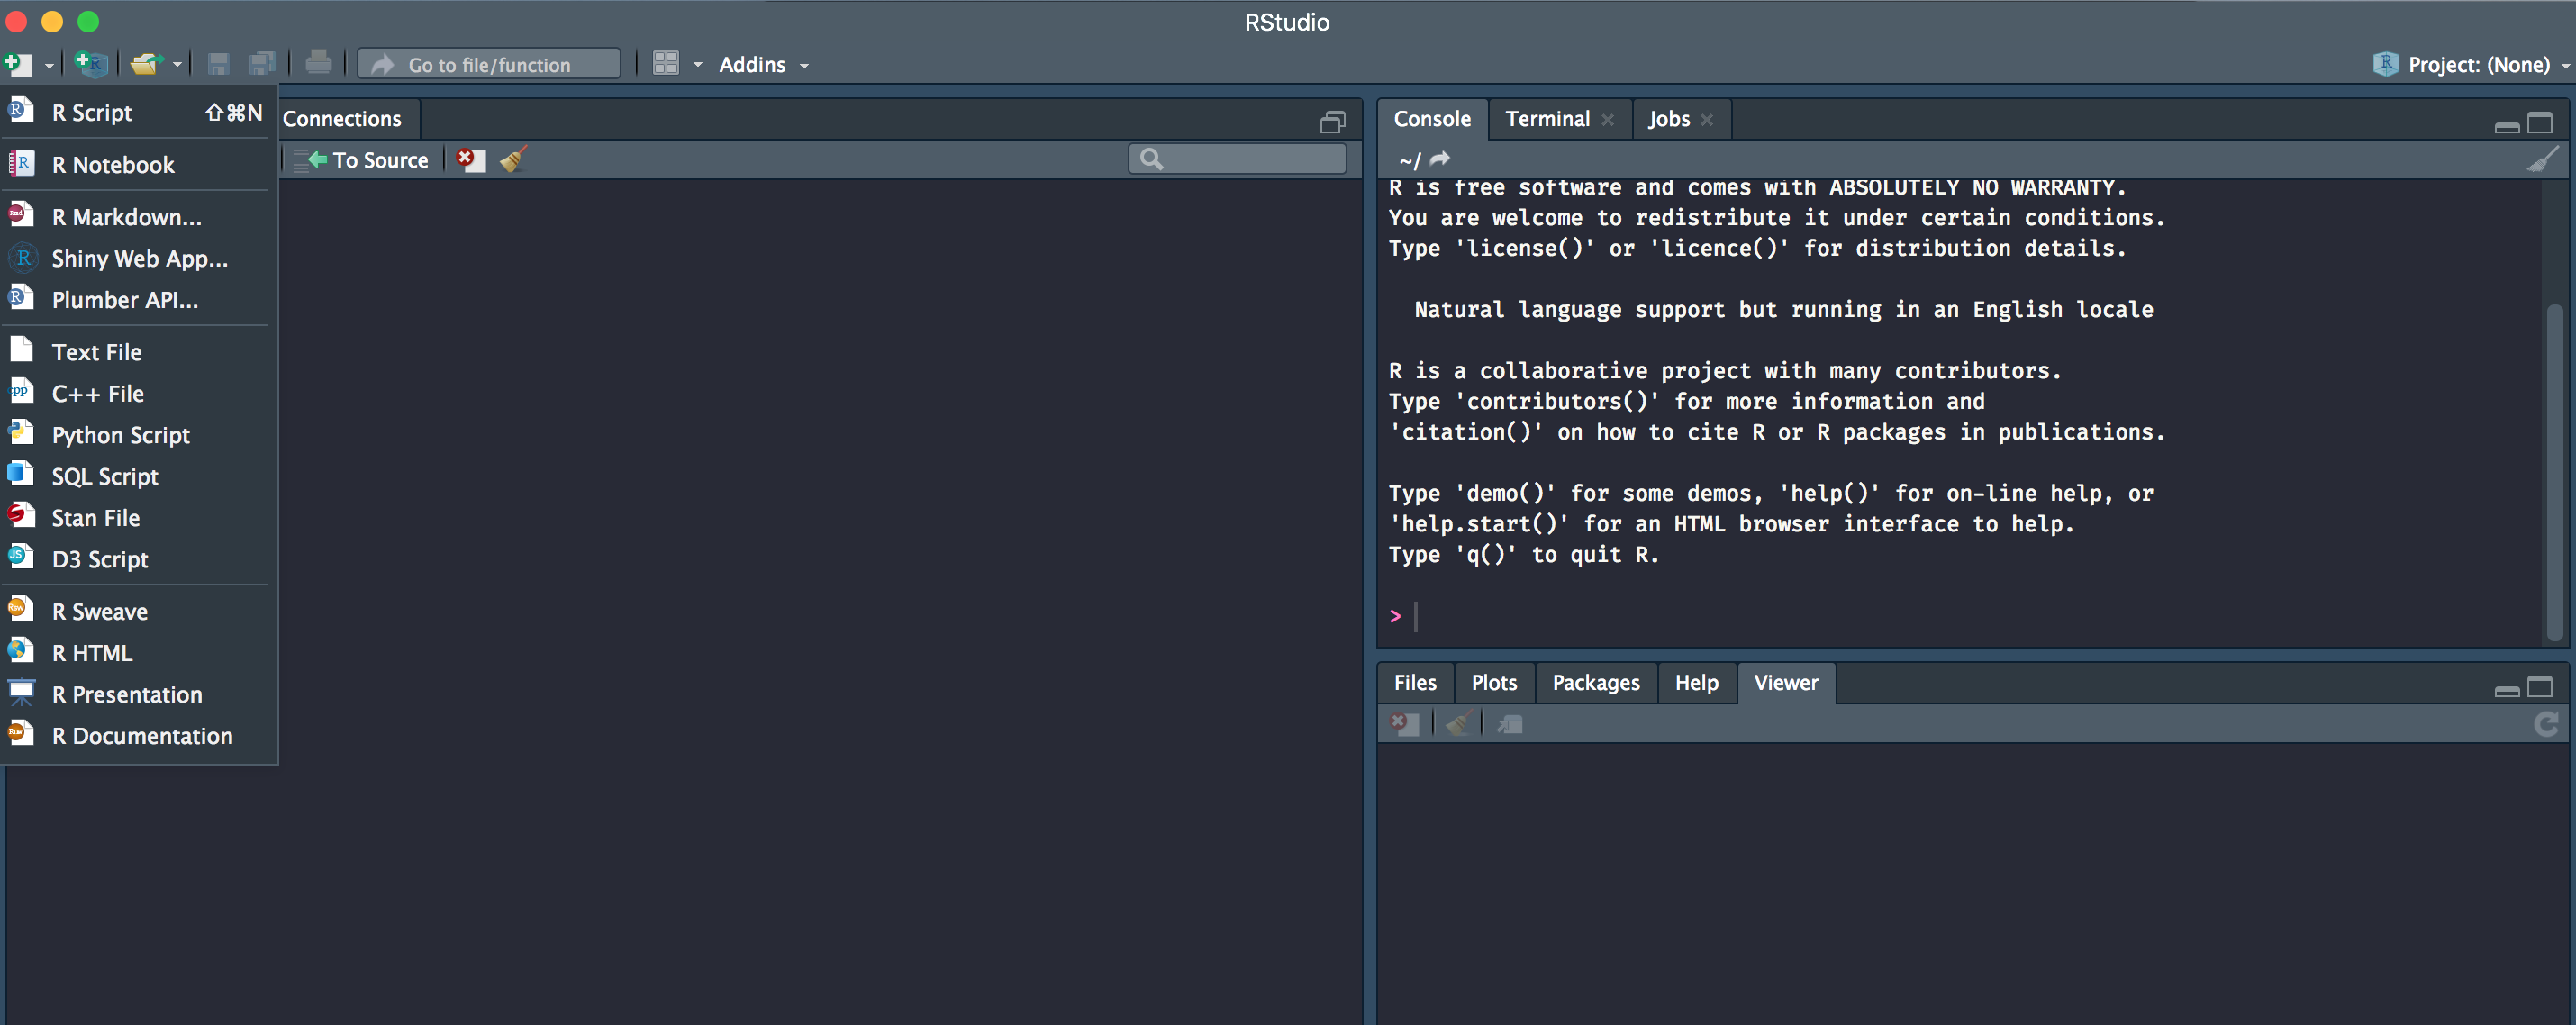
\includegraphics{img/OpenScript.png}

This opens up an R script file that you can edit and save. You will mainly be writing
in this panel within a R script (see \ref{workflow} for more details).

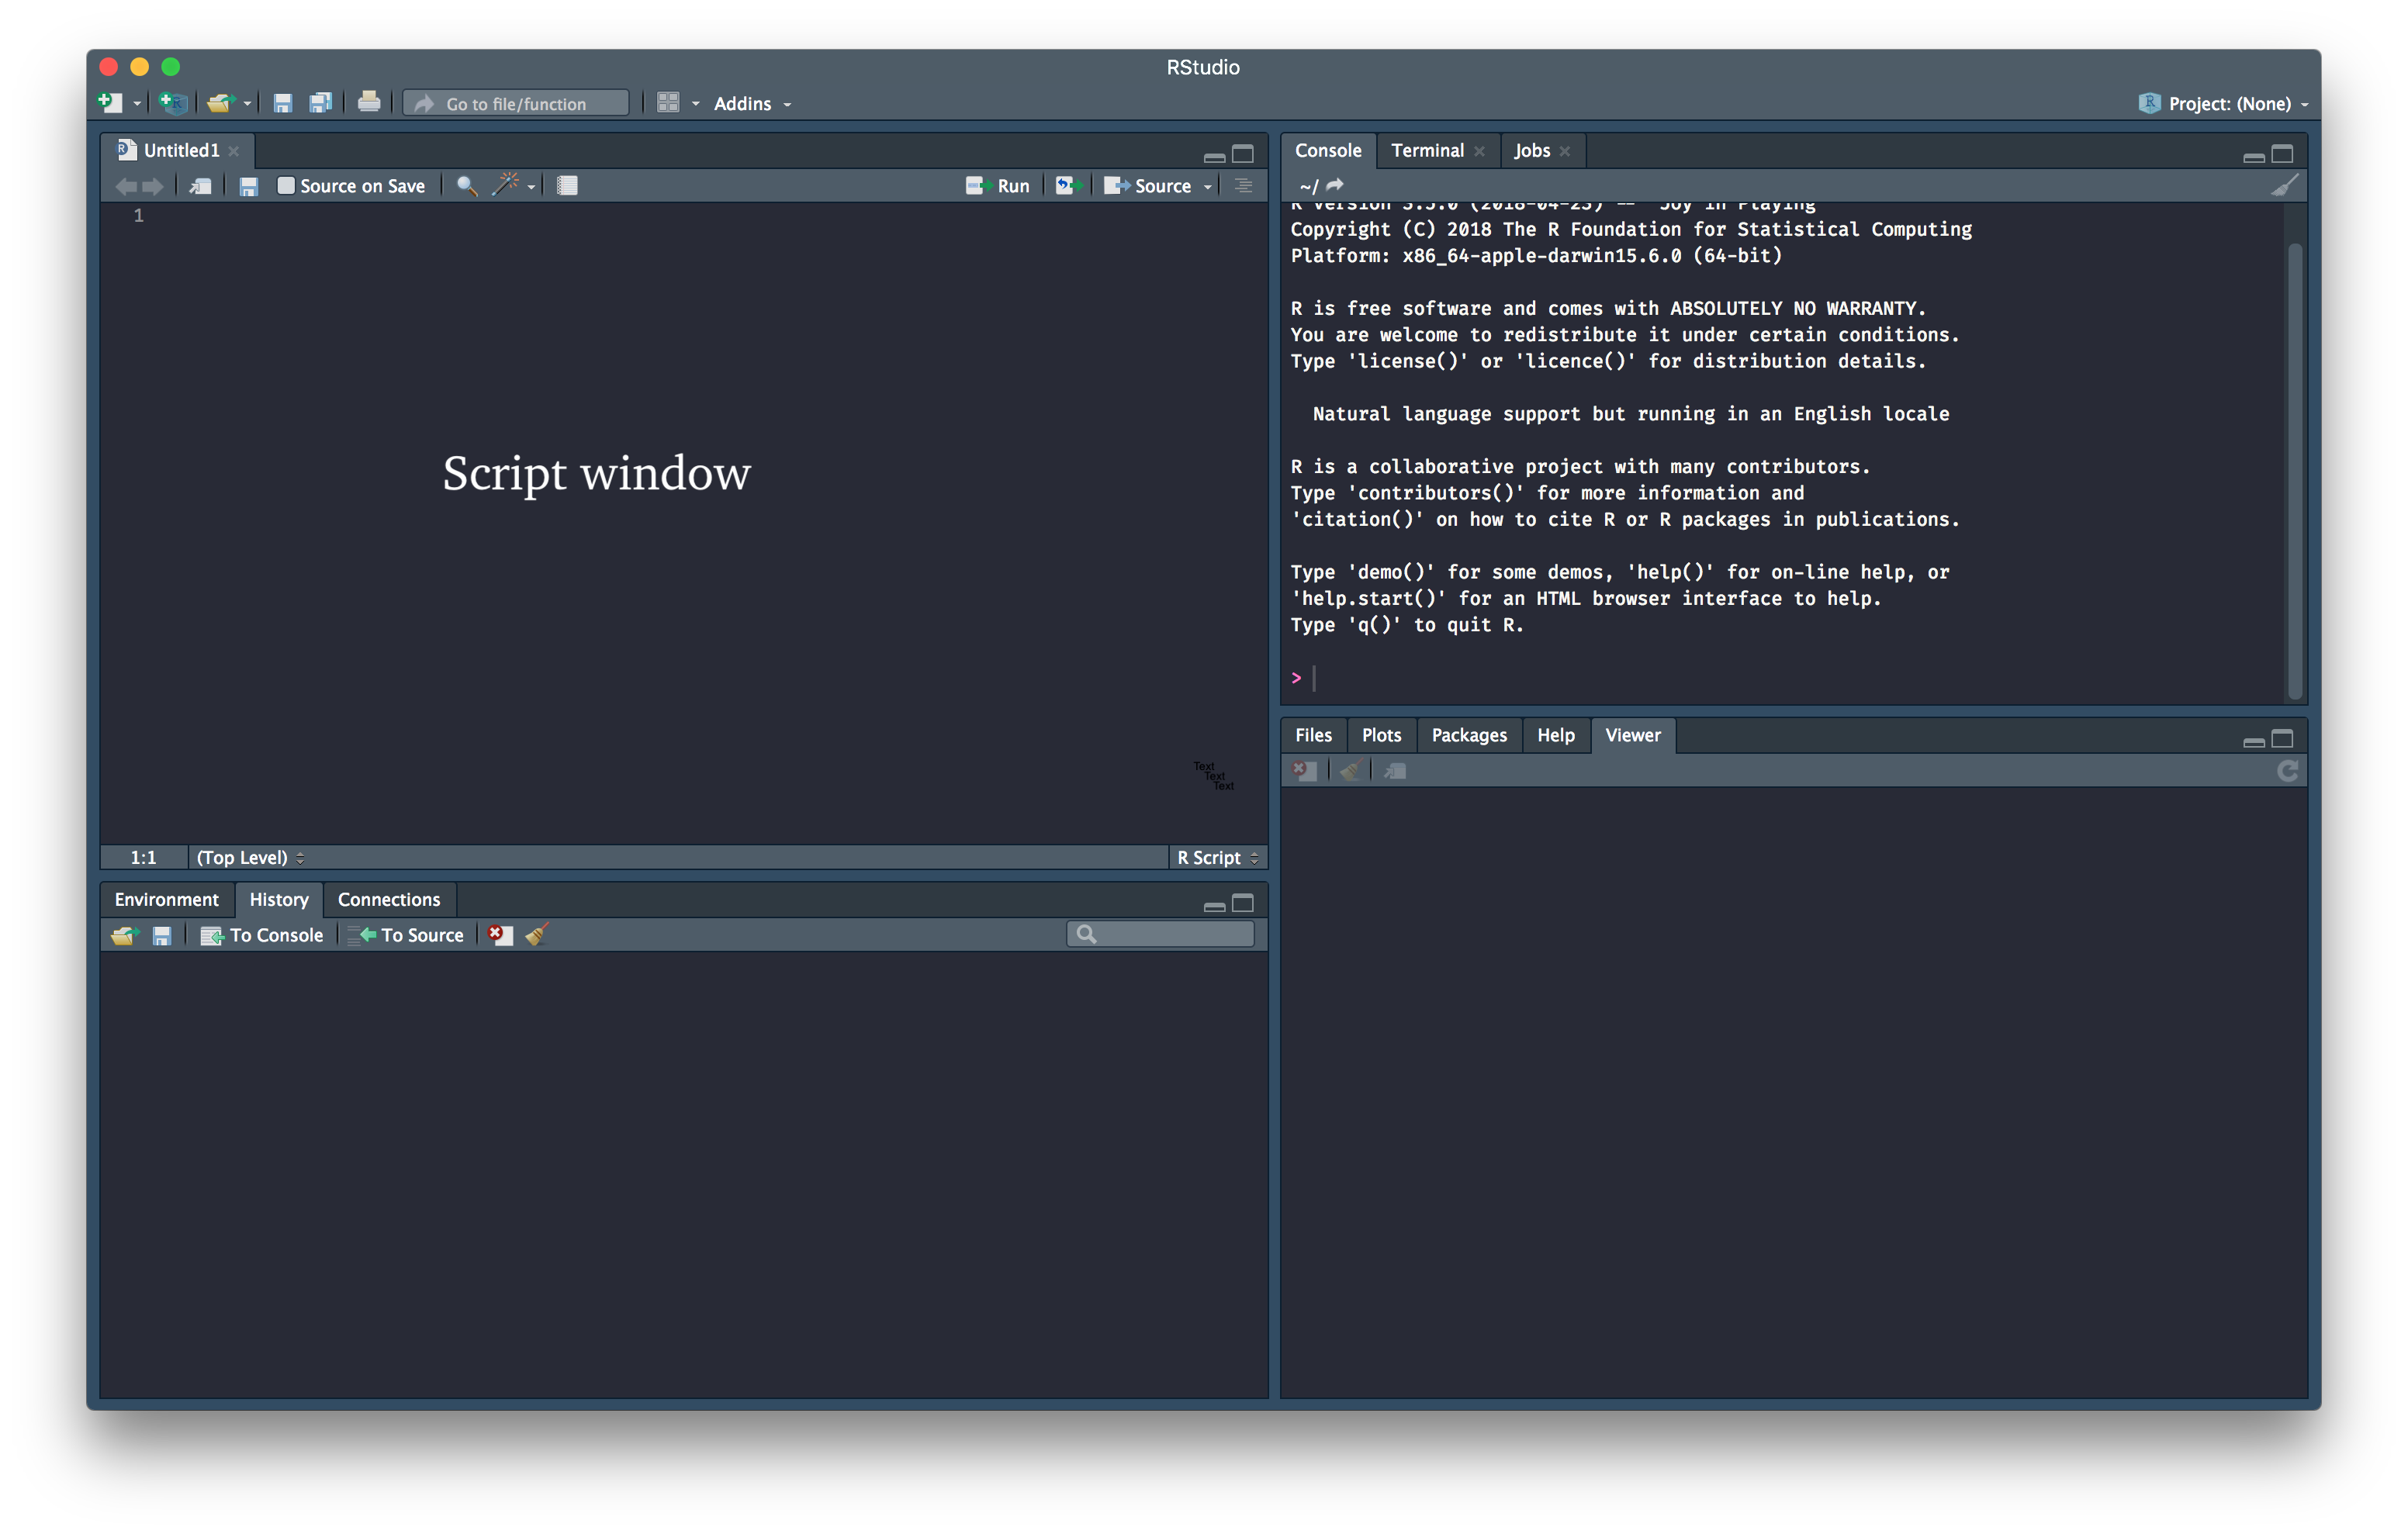
\includegraphics{img/ScriptPanel.png}

You will also have a Console panel where the code will actually run in R.

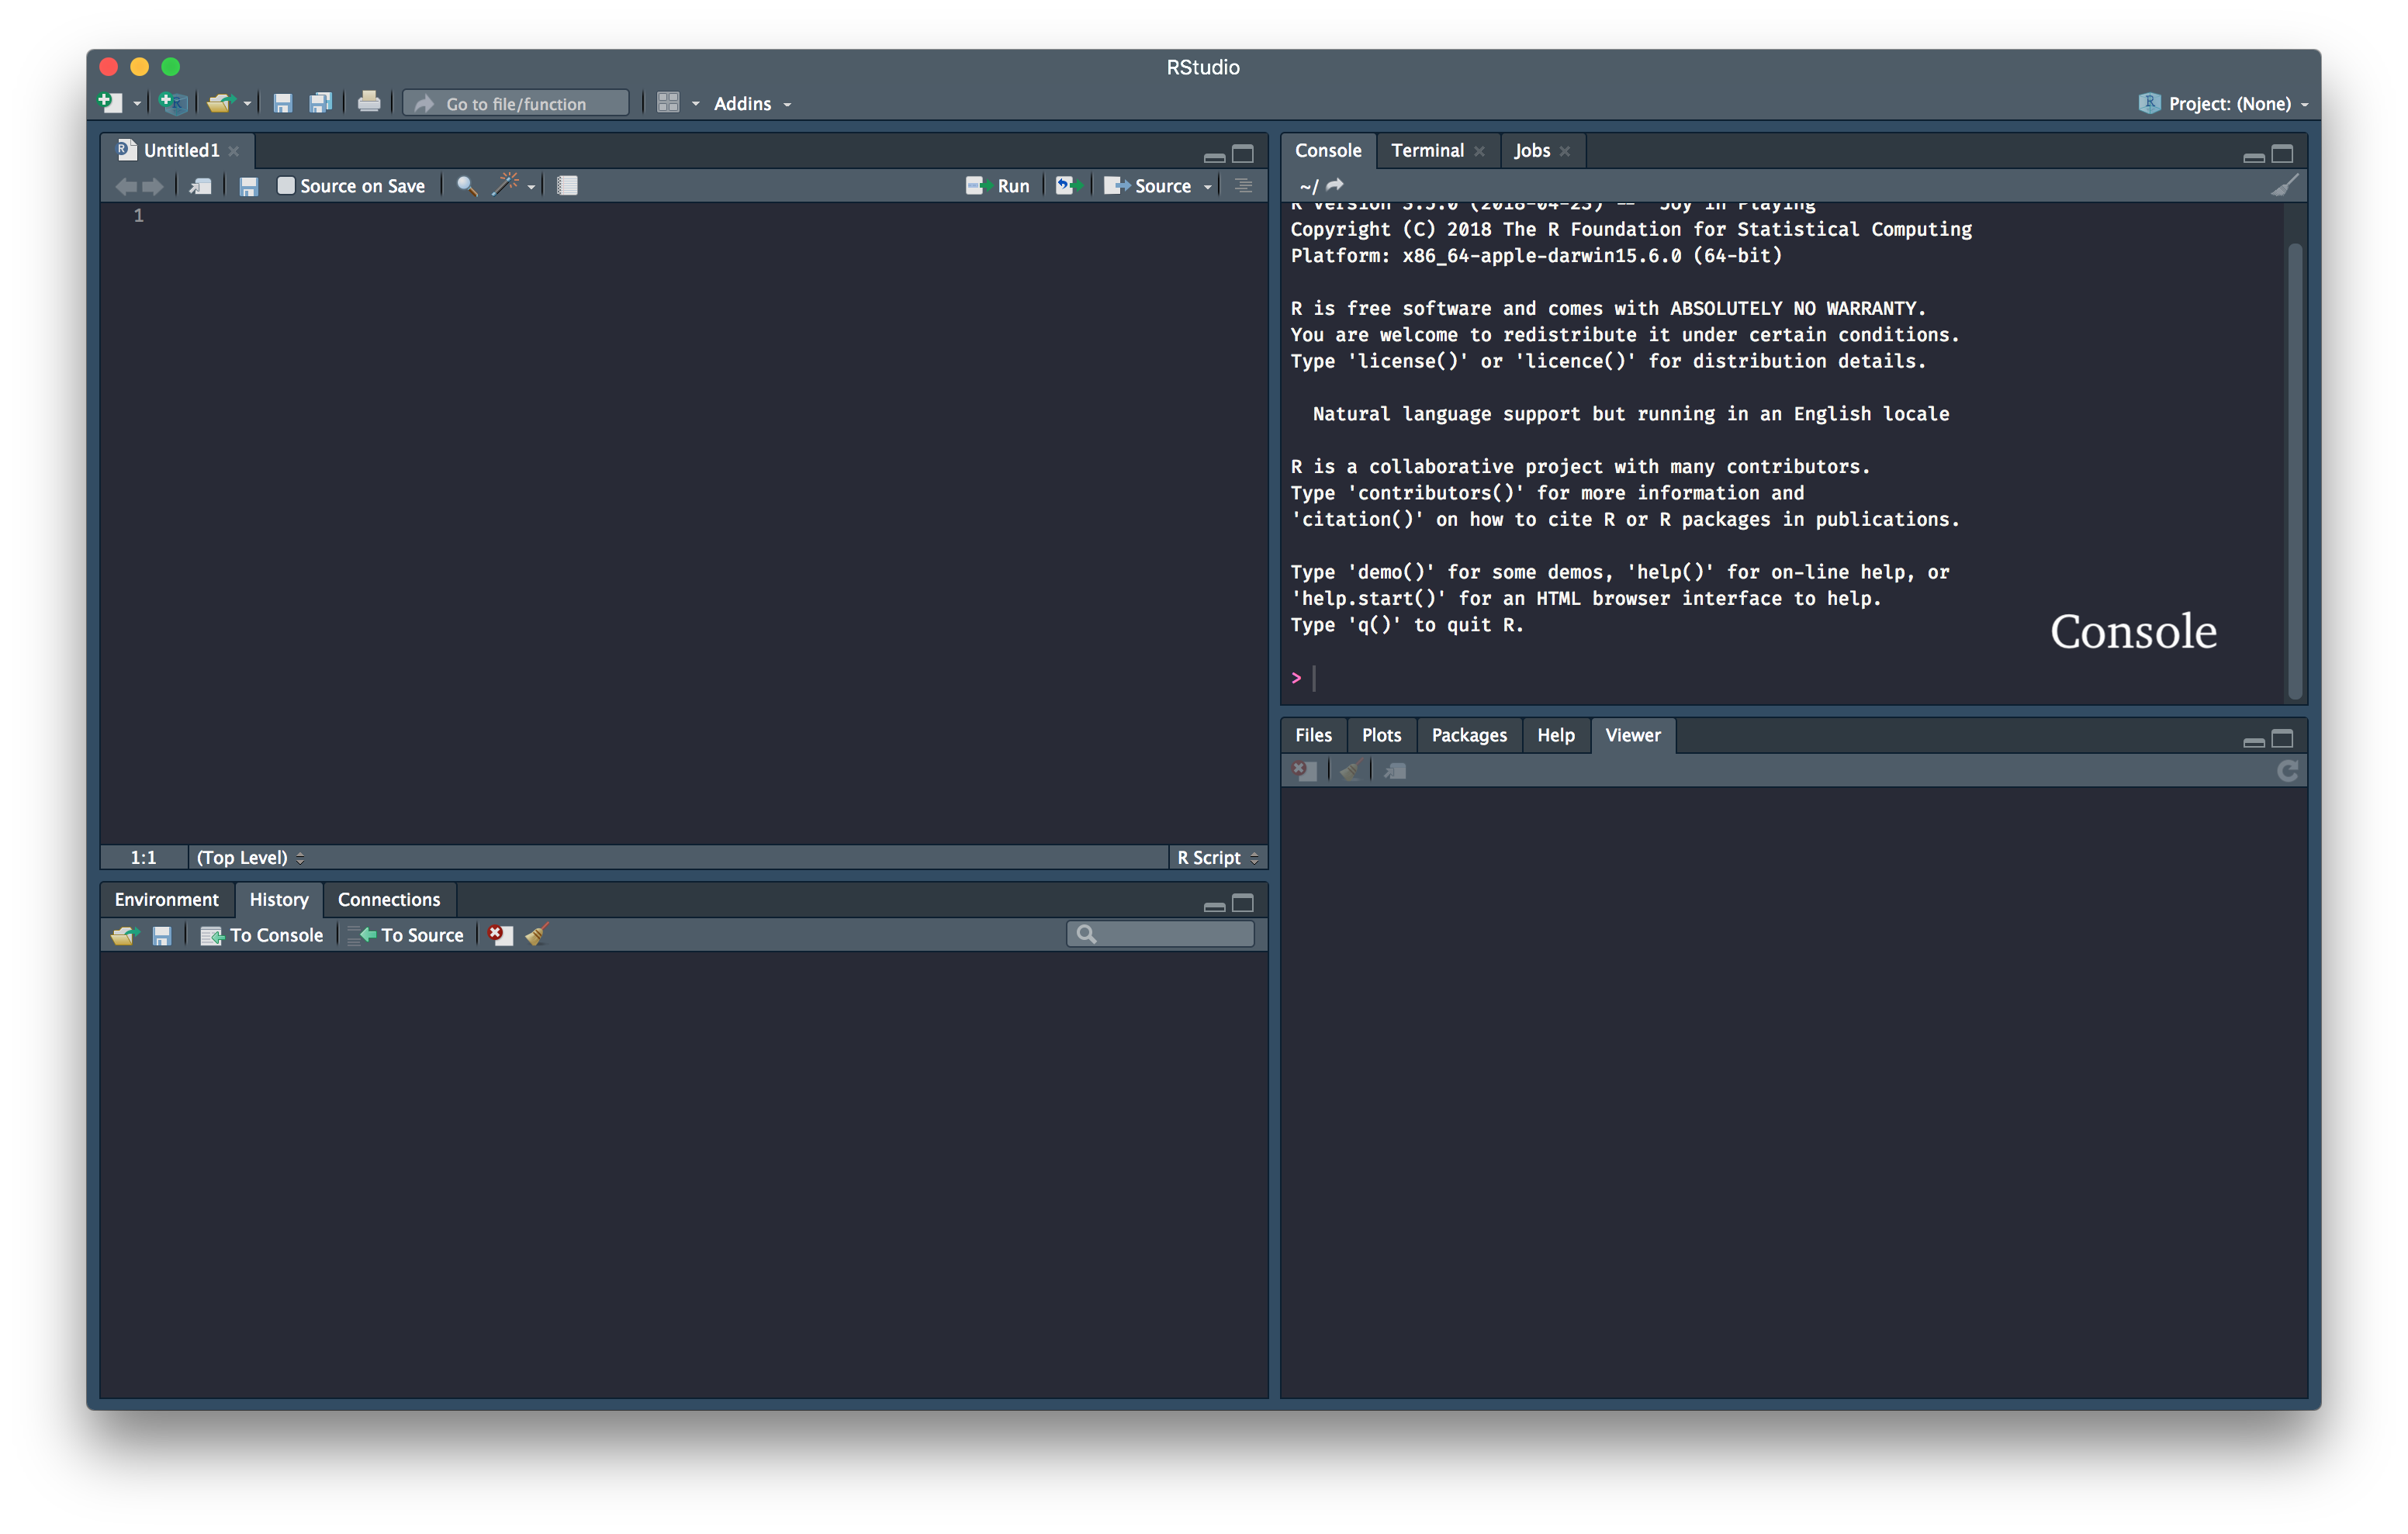
\includegraphics{img/ConsolePanel.png}

\hypertarget{other-panes}{%
\section*{Other panes}\label{other-panes}}
\addcontentsline{toc}{section}{Other panes}

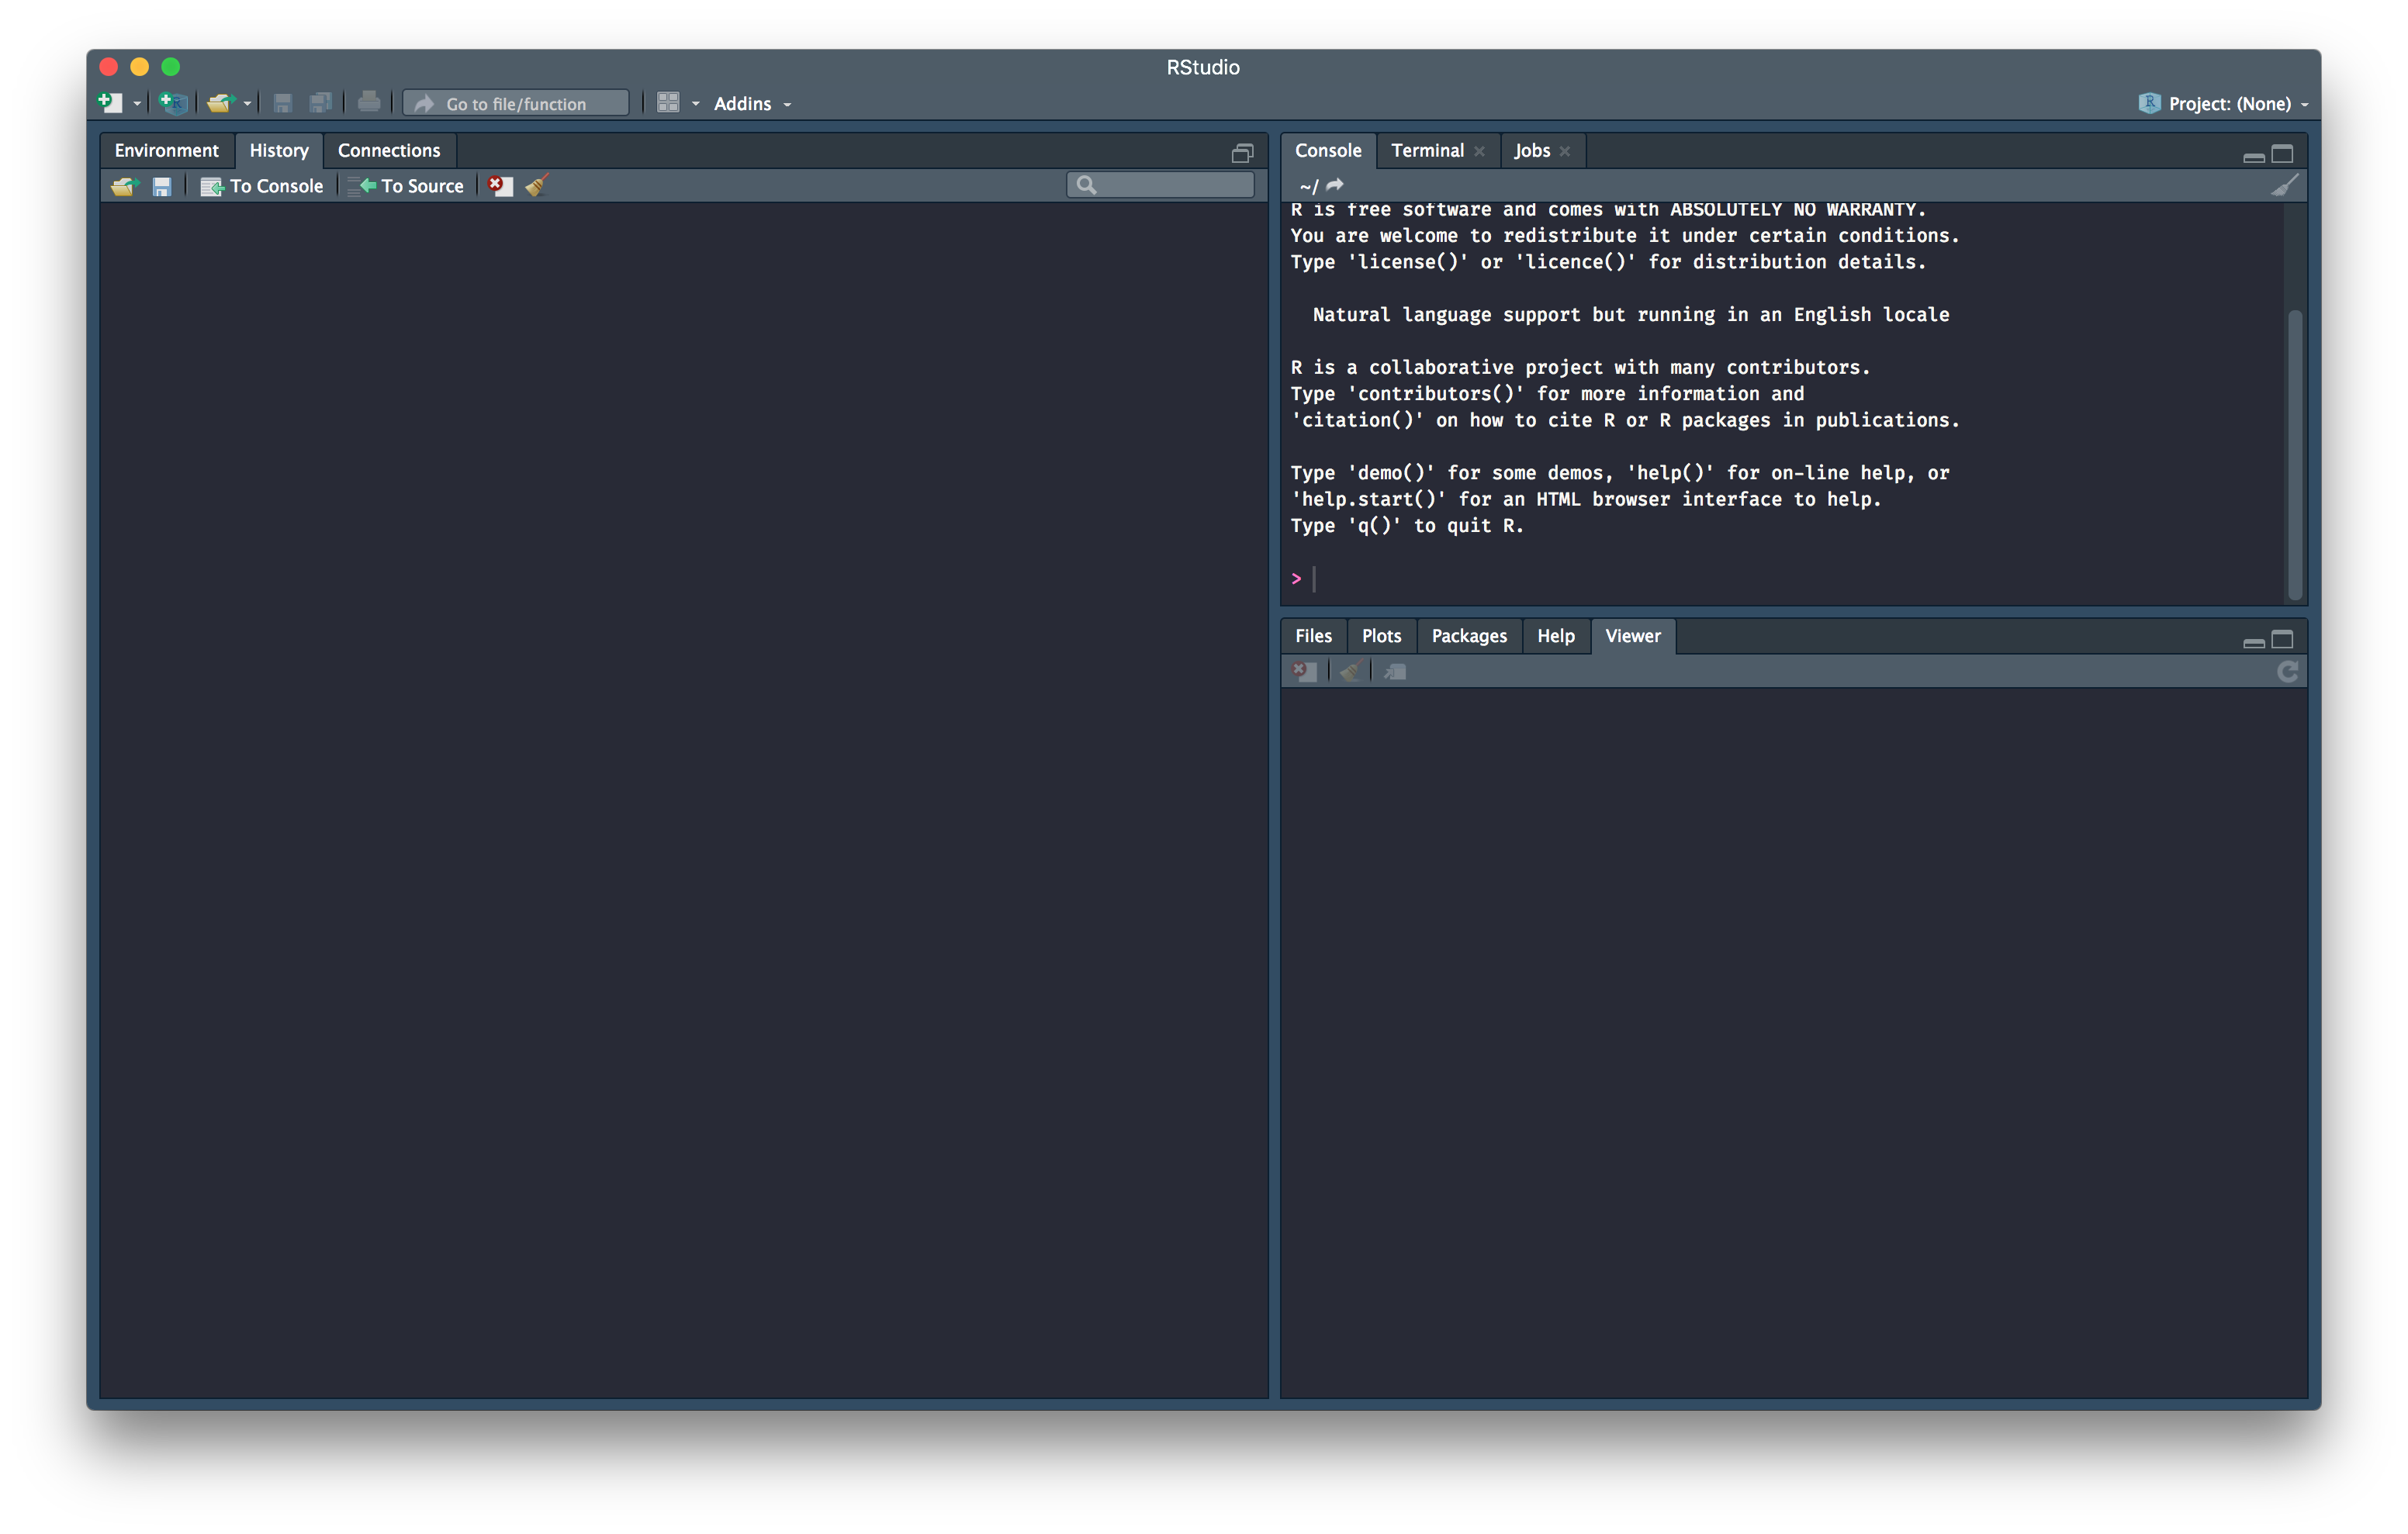
\includegraphics{img/RStudio.png}

There are several other panes in RStudio that we will see in due course.

\begin{itemize}
\tightlist
\item
  \textbf{Environment}: This shows all the objects (``words'') in your current environment
\item
  \textbf{History}: This gives a history of the commands you have run. This is searchable. Though
  you do have a stored history, see \ref{workflow} for why you shouldn't fall to temptation to
  just code in the console.
\item
  \textbf{Files}: This is exactly like File Explorer in Windows, and lets you see the contents of
  a folder/directory
\item
  \textbf{Plot}: These is where the plots will show up. See \ref{graphics} for more details on how to create plots
\item
  \textbf{Packages}: This gives a listing of installed packages. You \emph{can} click on the tick boxes to
  load packages into your environment, but I prefer coding it in (see section \ref{pkg}) to make it
  reproducible and verifiable.
\item
  \textbf{Help}: This will show help files once they are evoked
\item
  \textbf{Viewer}: This pane shows results when they are produced as HTML documents. This pane
  will also come into play once we start with interactive visualizations in section \ref{interactive}.
\end{itemize}

Feel free to explore these different panes and understand their functionalities.

\hypertarget{workflow}{%
\section{Rstudio workflow}\label{workflow}}

As we've seen, RStudio has both a scripting pane to write code, and a console pane to run code. Of course, you can write code directly into the console, but it is \textbf{not} a good practice. You will tend to get sloppy, lose the ``story'', and generally have less reproducible code.

Writing the program (``story'') is just more reliable if you write into the script file and the send it to the console to run. Sending it to the console can be acheieved with a keyboard shortcut, Ctrl-Enter (or Cmd-Enter on a Mac). This is something that will be second nature while coding in RStudio.

When you write code, be sure to comment your code liberally. In R, any line or any phrase starting with \texttt{\#} is considered a comment and is ignored by the program. This allows you to comment your code, explain your ideas to yourself and generally make your code more readable. To further this goal, write your code in differnt lines, and indent, to make it more readable; R ignores white space in your file.

Why bother doing this? Basically because the most likely next person to see your code is going to be you in 6 months, and you don't want to be scratching your head wondering what you were doing earlier (been there, done that, don't like it). You certainly can't phone your earlier self, so the best strategy is to write comments for your future self to minimize future grief.

\hypertarget{rstudio-projects}{%
\section{RStudio Projects}\label{rstudio-projects}}

Projects are a nice way to organize your data projects within RStudio. Projects keep together input data, R scripts, analytical results, and figures, and keeps different projects separate. Each project can run on its own independent R session (no worries about cross-hybridization), and you can have several projects open concurrently without risk of cross-pollinating them.

To make a new project, click \texttt{File\ \textgreater{}\ New\ Project}, then:

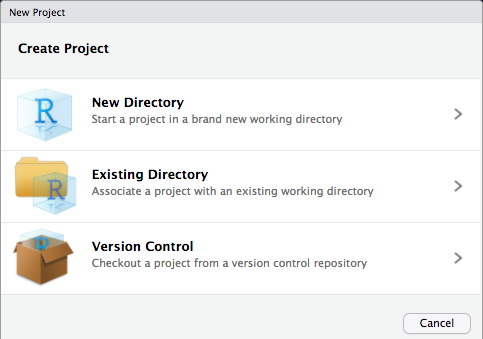
\includegraphics{img/Project2.png}
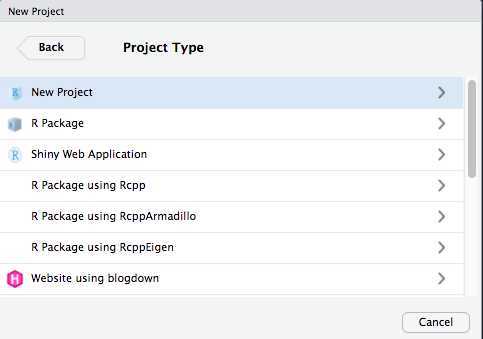
\includegraphics{img/Project3.png}
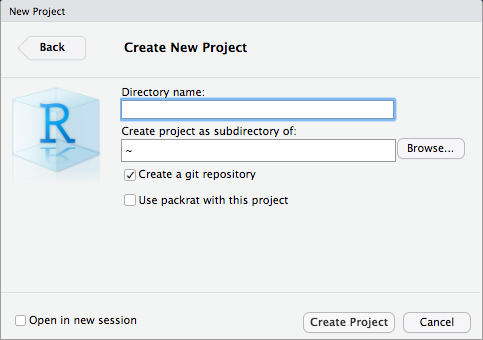
\includegraphics{img/Project1.png}

Note that I always create a git repository for version control. If you're not doing that,
untick the box in the window above.

\hypertarget{loading-data-into-r}{%
\chapter{Loading data into R}\label{loading-data-into-r}}

R can access data files from a wide variety of sources. These include

\begin{enumerate}
\def\labelenumi{\arabic{enumi}.}
\tightlist
\item
  Text files (csv, tsv, fixed-width)
\item
  Microsoft Excel files
\item
  Microsoft Access databases
\item
  SQL-based databases (MySql, Postgresql, SQLite, Amazon Redshift)
\item
  Enterprise databases (SAP, Oracle)
\end{enumerate}

The R package \texttt{rio} can help read and write to many file types that are single files,
and the package \texttt{rodbc} can do the same for the databases.

 \textbf{Exercise:} Install the R package \texttt{rio} into your R installation

\begin{Shaded}
\begin{Highlighting}[]
\KeywordTok{install.packages}\NormalTok{(}\StringTok{"rio"}\NormalTok{, }\DataTypeTok{repos =} \StringTok{"https://cran.rstudio.com"}\NormalTok{) }\CommentTok{# Note the quotes}
\end{Highlighting}
\end{Shaded}

The \texttt{rio} package has a common way of reading data (using the \texttt{import} function).
Importing the data will create an object called a data.frame, but if you
just import data, it is not saved since it doesn't yet have a name.

\begin{Shaded}
\begin{Highlighting}[]
\KeywordTok{library}\NormalTok{(rio) }\CommentTok{# activate the package}
\KeywordTok{import}\NormalTok{(}\StringTok{'data/HR_Data.csv'}\NormalTok{) }\CommentTok{# can use single or double quotes}
\end{Highlighting}
\end{Shaded}

So every time you import data, you have to name it. You do this using the \texttt{\textless{}-} operator.

\begin{Shaded}
\begin{Highlighting}[]
\NormalTok{hr_data <-}\StringTok{ }\KeywordTok{import}\NormalTok{(}\StringTok{'data/HR_Data.csv'}\NormalTok{)}
\end{Highlighting}
\end{Shaded}

Now, if you type \texttt{hr\_data} in the console, you will see the data you imported.

\begin{Shaded}
\begin{Highlighting}[]
\KeywordTok{head}\NormalTok{(hr_data) }\CommentTok{# This just displays the first 10 lines of the data}
\end{Highlighting}
\end{Shaded}

\begin{verbatim}
##                                                Bureau Gender Grade
## 1    Comptroller and Global Financial Services (CGFS) female   N/A
## 2                East Asian and Pacific Affairs (EAP) female   N/A
## 3                 Overseas Buildings Operations (OBO)   male  FS-5
## 4         Conflict and Stabilization Operations (CSO)   male   N/A
## 5                               Consular Affairs (CA) female  FS-5
## 6 Management Policy, Rightsizing and Innovation (PRI) female  FS-2
##             Name
## 1  Katrina Lilly
## 2          Keene
## 3 Garrett Murphy
## 4     Jim Rhodes
## 5    Anita Myers
## 6 Vivian Einhorn
##                                                                                           Skills
## 1                                   Hydrology, Research, Design, human resources, Administration
## 2                                                                           Sharepoint, Planning
## 3                interagency, Portuguese, Management, Foreign Policy, Economics, Human Resources
## 4                   education, seo, German, Finance, design, portuguese, disease response, Excel
## 5 Healthcare, training, German, french, Sharepoint, Marketing, Data Analysis, Economics, spanish
## 6                 data analysis, Web Development, Hydrology, IT, SEO, Disease Response, Japanese
##   YearsService
## 1           16
## 2           21
## 3            5
## 4            4
## 5           23
## 6           19
\end{verbatim}

Seeing the data like this is certainly a bit awkward, especially for large datasets.
In RStudio, you can see the data somewhat like a spreadsheet with the following command:

\begin{Shaded}
\begin{Highlighting}[]
\KeywordTok{View}\NormalTok{(hr_data)}
\end{Highlighting}
\end{Shaded}

This results in a new pane in RStudio.

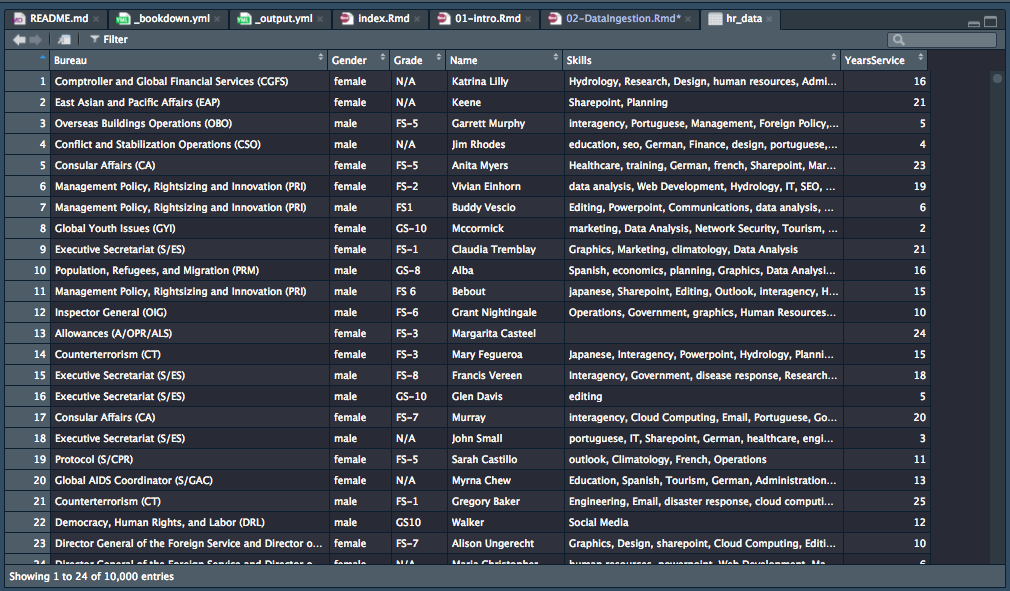
\includegraphics{img/Viewer.png}

\hypertarget{finer-control-of-csv-imports}{%
\section{Finer control of CSV imports}\label{finer-control-of-csv-imports}}

We can provide finer control over importing text files using additional options (``adverbs'') to
the \texttt{import} function (``verb''). For example, it might be good to check if all the column
names are unique, and to make them not have spaces (which are awkward in terms of typing and functionality). You can add the option \texttt{check.names\ =\ TRUE} to the command:

\begin{Shaded}
\begin{Highlighting}[]
\NormalTok{hr_data <-}\StringTok{ }\KeywordTok{import}\NormalTok{(}\StringTok{'data/HR_Data.csv'}\NormalTok{, }\DataTypeTok{check.names =} \OtherTok{TRUE}\NormalTok{)}
\end{Highlighting}
\end{Shaded}

Similarly, if you're using European data, where the decimal point is denoted by a comma, you can
add the following option:

\begin{Shaded}
\begin{Highlighting}[]
\NormalTok{hr_data <-}\StringTok{ }\KeywordTok{import}\NormalTok{(}\StringTok{'data/HR_Data.csv'}\NormalTok{, }\DataTypeTok{check.names =} \OtherTok{TRUE}\NormalTok{, }\DataTypeTok{dec =} \StringTok{','}\NormalTok{)}
\end{Highlighting}
\end{Shaded}

You can see most of the options in the help file for import, which you can access
either from the \texttt{Help} pane, or by typing \texttt{?import} or \texttt{help(import)} in the console

\hypertarget{finer-control-of-excel-imports}{%
\section{Finer control of Excel imports}\label{finer-control-of-excel-imports}}

You can specify sheet names or sheet positions for import from an Excel file. If you
know the sheet name, you can specify it using the \texttt{which} option:

\begin{Shaded}
\begin{Highlighting}[]
\NormalTok{dos_data <-}\StringTok{ }\KeywordTok{import}\NormalTok{(}\StringTok{'data/simulatedDOS.xlsx'}\NormalTok{, }\DataTypeTok{which=}\StringTok{'Staffing_by_Bureau'}\NormalTok{)}
\end{Highlighting}
\end{Shaded}

You can also grab the same sheet by position:

\begin{Shaded}
\begin{Highlighting}[]
\NormalTok{dos_data <-}\StringTok{ }\KeywordTok{import}\NormalTok{(}\StringTok{'data/simulatedDOS.xlsx'}\NormalTok{, }\DataTypeTok{which =} \DecValTok{2}\NormalTok{)}
\end{Highlighting}
\end{Shaded}

We'll talk about how to grab multiple sheets together into a list in the data munging section\ref{sec:data-munging}.

\hypertarget{importing-data-from-databases}{%
\section{Importing data from databases}\label{importing-data-from-databases}}

If you have data in an Access database, you can read it in pretty easily using
the \texttt{RODBC} package. To import one particular table from Access, you can use

\begin{Shaded}
\begin{Highlighting}[]
\KeywordTok{library}\NormalTok{(RODBC) }\CommentTok{# activate package, case-sensitive}
\NormalTok{channel <-}\StringTok{ }\KeywordTok{odbcConnectAccess}\NormalTok{(}\StringTok{'C:/Documents/Name_of_Access_Database'}\NormalTok{) }\CommentTok{# change to your}
\NormalTok{mydata <-}\StringTok{ }\KeywordTok{sqlQuery}\NormalTok{(channel, }\KeywordTok{paste}\NormalTok{(}\StringTok{"select * from Name_of_table_in_database"}\NormalTok{))}
\end{Highlighting}
\end{Shaded}

For other databases, the connection can be made using the \texttt{odbc} package. You can connnect
to a MySQL database, for example, using

\begin{Shaded}
\begin{Highlighting}[]
\KeywordTok{library}\NormalTok{(odbc)}
\NormalTok{con <-}\StringTok{ }\KeywordTok{dbConnect}\NormalTok{(}\KeywordTok{odbc}\NormalTok{(),}
                 \DataTypeTok{Driver   =} \StringTok{"[your driver's name]"}\NormalTok{,}
                 \DataTypeTok{Server   =} \StringTok{"[your server's path]"}\NormalTok{,}
                 \DataTypeTok{Database =} \StringTok{"[your database's name]"}\NormalTok{,}
                 \DataTypeTok{UID      =}\NormalTok{ rstudioapi}\OperatorTok{::}\KeywordTok{askForPassword}\NormalTok{(}\StringTok{"Database user"}\NormalTok{),}
                 \DataTypeTok{PWD      =}\NormalTok{ rstudioapi}\OperatorTok{::}\KeywordTok{askForPassword}\NormalTok{(}\StringTok{"Database password"}\NormalTok{),}
                 \DataTypeTok{Port     =} \DecValTok{1433}\NormalTok{)}
\end{Highlighting}
\end{Shaded}

and you can load a table into R using

\begin{Shaded}
\begin{Highlighting}[]
\NormalTok{dat <-}\StringTok{ }\KeywordTok{dbGetQuery}\NormalTok{(con, }\StringTok{'select * from <table name>'}\NormalTok{)}
\end{Highlighting}
\end{Shaded}

You'll notice that it is a bit more complicated to call data from databases, though
once it's set up, it works beautifully. For more details about this process for different
databases, see \href{https://db.rstudio.com/}{RStudio's tutorial}.

\hypertarget{sec:data-munging}{%
\chapter{Data Munging}\label{sec:data-munging}}

Data munging refers to the work of transforming data to make it usable for a computer.
Data unfortunately comes in all shapes and sizes, with all sorts of issues, so this
process can take a while. Often a rule of thumb is that making a data set ready for
analysis takes about 80\% of the time of a project.

\hypertarget{tidy-data}{%
\section{Tidy data}\label{tidy-data}}

There is a principle of making data ``tidy'', promoted by Dr.~Hadley Wickham. This
tidying of data makes computer programs happy, since these data can be most
easily digested. A dataset can be messy or tidy depending on how the rows, columns and tables you're
using align with observations, variables and types.

The properties of a tidy dataset are:

\begin{enumerate}
\def\labelenumi{\arabic{enumi}.}
\tightlist
\item
  Each variable forms a column
\item
  Each observation forms a row
\item
  Each type of observational unit forms a table.
\end{enumerate}

This forms a standardized way to structure a dataset, and so makes it easy for the
analyst to develop standard pipelines.

A dataset can be messy in many many ways. Many of the more common issues are listed below:

\begin{itemize}
\tightlist
\item
  Column names contain values, not just variable names
\item
  Multiple variables are stored in one column
\item
  Variables are stored in both rows and columns
\item
  Multiple types of observational types are stored in the same table
\item
  A single observational unit is stored in multiple tables
\end{itemize}

Sometimes the messier format is better for data entry, but bad for data analyses.

We'll show a few examples here, but a more detailed discussion is available \href{https://cran.r-project.org/web/packages/tidyr/vignettes/tidy-data.html}{online}.

The workhorse for this tidying activity is the \texttt{tidyr} package, part of the \texttt{tidyverse}
meta-package. We'll tend to start every analysis by loading the \texttt{tidyverse} package,
so we are covered.

\hypertarget{variable-in-column-names}{%
\subsection{Variable in column names}\label{variable-in-column-names}}

\begin{Shaded}
\begin{Highlighting}[]
\KeywordTok{library}\NormalTok{(tidyverse)}
\end{Highlighting}
\end{Shaded}

\begin{verbatim}
## -- Attaching packages --------------------------------------------------------------------------------- tidyverse 1.2.1 --
\end{verbatim}

\begin{verbatim}
## v ggplot2 3.1.0          v purrr   0.3.2     
## v tibble  2.0.1          v dplyr   0.8.0.9009
## v tidyr   0.8.3          v stringr 1.4.0     
## v readr   1.3.1          v forcats 0.4.0
\end{verbatim}

\begin{verbatim}
## Warning: package 'tibble' was built under R version 3.5.2
\end{verbatim}

\begin{verbatim}
## Warning: package 'tidyr' was built under R version 3.5.2
\end{verbatim}

\begin{verbatim}
## Warning: package 'stringr' was built under R version 3.5.2
\end{verbatim}

\begin{verbatim}
## -- Conflicts ------------------------------------------------------------------------------------ tidyverse_conflicts() --
## x dplyr::filter() masks stats::filter()
## x dplyr::lag()    masks stats::lag()
\end{verbatim}

\begin{Shaded}
\begin{Highlighting}[]
\NormalTok{pew <-}\StringTok{ }\KeywordTok{import}\NormalTok{(}\StringTok{'data/pew.csv'}\NormalTok{)}
\KeywordTok{head}\NormalTok{(pew)}
\end{Highlighting}
\end{Shaded}

\begin{verbatim}
##             religion <$10k $10-20k $20-30k $30-40k $40-50k $50-75k
## 1           Agnostic    27      34      60      81      76     137
## 2            Atheist    12      27      37      52      35      70
## 3           Buddhist    27      21      30      34      33      58
## 4           Catholic   418     617     732     670     638    1116
## 5 Don’t know/refused    15      14      15      11      10      35
## 6   Evangelical Prot   575     869    1064     982     881    1486
##   $75-100k $100-150k >150k Don't know/refused
## 1      122       109    84                 96
## 2       73        59    74                 76
## 3       62        39    53                 54
## 4      949       792   633               1489
## 5       21        17    18                116
## 6      949       723   414               1529
\end{verbatim}

This dataset has actual data in the column headers, rather than variable names. This
information needs to be captured into a column. We should ideally have 3 columns in this
dataset: religion, income and frequency. We can achieve this using a function called \texttt{gather} which
takes a wide dataset and makes it tall. We will do this by forming a pipeline (think of this as a sentence),
starting with the dataset.

\begin{Shaded}
\begin{Highlighting}[]
\NormalTok{pew }\OperatorTok\StringTok{ }
\StringTok{  }\KeywordTok{gather}\NormalTok{(income, frequency, }\OperatorTok{-}\NormalTok{religion)}
\end{Highlighting}
\end{Shaded}

\begin{verbatim}
##                    religion             income frequency
## 1                  Agnostic              <$10k        27
## 2                   Atheist              <$10k        12
## 3                  Buddhist              <$10k        27
## 4                  Catholic              <$10k       418
## 5        Don’t know/refused              <$10k        15
## 6          Evangelical Prot              <$10k       575
## 7                     Hindu              <$10k         1
## 8   Historically Black Prot              <$10k       228
## 9         Jehovah's Witness              <$10k        20
## 10                   Jewish              <$10k        19
## 11            Mainline Prot              <$10k       289
## 12                   Mormon              <$10k        29
## 13                   Muslim              <$10k         6
## 14                 Orthodox              <$10k        13
## 15          Other Christian              <$10k         9
## 16             Other Faiths              <$10k        20
## 17    Other World Religions              <$10k         5
## 18             Unaffiliated              <$10k       217
## 19                 Agnostic            $10-20k        34
## 20                  Atheist            $10-20k        27
## 21                 Buddhist            $10-20k        21
## 22                 Catholic            $10-20k       617
## 23       Don’t know/refused            $10-20k        14
## 24         Evangelical Prot            $10-20k       869
## 25                    Hindu            $10-20k         9
## 26  Historically Black Prot            $10-20k       244
## 27        Jehovah's Witness            $10-20k        27
## 28                   Jewish            $10-20k        19
## 29            Mainline Prot            $10-20k       495
## 30                   Mormon            $10-20k        40
## 31                   Muslim            $10-20k         7
## 32                 Orthodox            $10-20k        17
## 33          Other Christian            $10-20k         7
## 34             Other Faiths            $10-20k        33
## 35    Other World Religions            $10-20k         2
## 36             Unaffiliated            $10-20k       299
## 37                 Agnostic            $20-30k        60
## 38                  Atheist            $20-30k        37
## 39                 Buddhist            $20-30k        30
## 40                 Catholic            $20-30k       732
## 41       Don’t know/refused            $20-30k        15
## 42         Evangelical Prot            $20-30k      1064
## 43                    Hindu            $20-30k         7
## 44  Historically Black Prot            $20-30k       236
## 45        Jehovah's Witness            $20-30k        24
## 46                   Jewish            $20-30k        25
## 47            Mainline Prot            $20-30k       619
## 48                   Mormon            $20-30k        48
## 49                   Muslim            $20-30k         9
## 50                 Orthodox            $20-30k        23
## 51          Other Christian            $20-30k        11
## 52             Other Faiths            $20-30k        40
## 53    Other World Religions            $20-30k         3
## 54             Unaffiliated            $20-30k       374
## 55                 Agnostic            $30-40k        81
## 56                  Atheist            $30-40k        52
## 57                 Buddhist            $30-40k        34
## 58                 Catholic            $30-40k       670
## 59       Don’t know/refused            $30-40k        11
## 60         Evangelical Prot            $30-40k       982
## 61                    Hindu            $30-40k         9
## 62  Historically Black Prot            $30-40k       238
## 63        Jehovah's Witness            $30-40k        24
## 64                   Jewish            $30-40k        25
## 65            Mainline Prot            $30-40k       655
## 66                   Mormon            $30-40k        51
## 67                   Muslim            $30-40k        10
## 68                 Orthodox            $30-40k        32
## 69          Other Christian            $30-40k        13
## 70             Other Faiths            $30-40k        46
## 71    Other World Religions            $30-40k         4
## 72             Unaffiliated            $30-40k       365
## 73                 Agnostic            $40-50k        76
## 74                  Atheist            $40-50k        35
## 75                 Buddhist            $40-50k        33
## 76                 Catholic            $40-50k       638
## 77       Don’t know/refused            $40-50k        10
## 78         Evangelical Prot            $40-50k       881
## 79                    Hindu            $40-50k        11
## 80  Historically Black Prot            $40-50k       197
## 81        Jehovah's Witness            $40-50k        21
## 82                   Jewish            $40-50k        30
## 83            Mainline Prot            $40-50k       651
## 84                   Mormon            $40-50k        56
## 85                   Muslim            $40-50k         9
## 86                 Orthodox            $40-50k        32
## 87          Other Christian            $40-50k        13
## 88             Other Faiths            $40-50k        49
## 89    Other World Religions            $40-50k         2
## 90             Unaffiliated            $40-50k       341
## 91                 Agnostic            $50-75k       137
## 92                  Atheist            $50-75k        70
## 93                 Buddhist            $50-75k        58
## 94                 Catholic            $50-75k      1116
## 95       Don’t know/refused            $50-75k        35
## 96         Evangelical Prot            $50-75k      1486
## 97                    Hindu            $50-75k        34
## 98  Historically Black Prot            $50-75k       223
## 99        Jehovah's Witness            $50-75k        30
## 100                  Jewish            $50-75k        95
## 101           Mainline Prot            $50-75k      1107
## 102                  Mormon            $50-75k       112
## 103                  Muslim            $50-75k        23
## 104                Orthodox            $50-75k        47
## 105         Other Christian            $50-75k        14
## 106            Other Faiths            $50-75k        63
## 107   Other World Religions            $50-75k         7
## 108            Unaffiliated            $50-75k       528
## 109                Agnostic           $75-100k       122
## 110                 Atheist           $75-100k        73
## 111                Buddhist           $75-100k        62
## 112                Catholic           $75-100k       949
## 113      Don’t know/refused           $75-100k        21
## 114        Evangelical Prot           $75-100k       949
## 115                   Hindu           $75-100k        47
## 116 Historically Black Prot           $75-100k       131
## 117       Jehovah's Witness           $75-100k        15
## 118                  Jewish           $75-100k        69
## 119           Mainline Prot           $75-100k       939
## 120                  Mormon           $75-100k        85
## 121                  Muslim           $75-100k        16
## 122                Orthodox           $75-100k        38
## 123         Other Christian           $75-100k        18
## 124            Other Faiths           $75-100k        46
## 125   Other World Religions           $75-100k         3
## 126            Unaffiliated           $75-100k       407
## 127                Agnostic          $100-150k       109
## 128                 Atheist          $100-150k        59
## 129                Buddhist          $100-150k        39
## 130                Catholic          $100-150k       792
## 131      Don’t know/refused          $100-150k        17
## 132        Evangelical Prot          $100-150k       723
## 133                   Hindu          $100-150k        48
## 134 Historically Black Prot          $100-150k        81
## 135       Jehovah's Witness          $100-150k        11
## 136                  Jewish          $100-150k        87
## 137           Mainline Prot          $100-150k       753
## 138                  Mormon          $100-150k        49
## 139                  Muslim          $100-150k         8
## 140                Orthodox          $100-150k        42
## 141         Other Christian          $100-150k        14
## 142            Other Faiths          $100-150k        40
## 143   Other World Religions          $100-150k         4
## 144            Unaffiliated          $100-150k       321
## 145                Agnostic              >150k        84
## 146                 Atheist              >150k        74
## 147                Buddhist              >150k        53
## 148                Catholic              >150k       633
## 149      Don’t know/refused              >150k        18
## 150        Evangelical Prot              >150k       414
## 151                   Hindu              >150k        54
## 152 Historically Black Prot              >150k        78
## 153       Jehovah's Witness              >150k         6
## 154                  Jewish              >150k       151
## 155           Mainline Prot              >150k       634
## 156                  Mormon              >150k        42
## 157                  Muslim              >150k         6
## 158                Orthodox              >150k        46
## 159         Other Christian              >150k        12
## 160            Other Faiths              >150k        41
## 161   Other World Religions              >150k         4
## 162            Unaffiliated              >150k       258
## 163                Agnostic Don't know/refused        96
## 164                 Atheist Don't know/refused        76
## 165                Buddhist Don't know/refused        54
## 166                Catholic Don't know/refused      1489
## 167      Don’t know/refused Don't know/refused       116
## 168        Evangelical Prot Don't know/refused      1529
## 169                   Hindu Don't know/refused        37
## 170 Historically Black Prot Don't know/refused       339
## 171       Jehovah's Witness Don't know/refused        37
## 172                  Jewish Don't know/refused       162
## 173           Mainline Prot Don't know/refused      1328
## 174                  Mormon Don't know/refused        69
## 175                  Muslim Don't know/refused        22
## 176                Orthodox Don't know/refused        73
## 177         Other Christian Don't know/refused        18
## 178            Other Faiths Don't know/refused        71
## 179   Other World Religions Don't know/refused         8
## 180            Unaffiliated Don't know/refused       597
\end{verbatim}

Let's parse this out. First we see this new operator \texttt{\%\textgreater{}\%}, which you can think of as the word ``then''.
So we start with the dataset \texttt{pew}, ``then'' we gather its columns into two columns, \texttt{income} and \texttt{frequency}.
We don't want the \texttt{religion} column to be part of this operation, so we ``minus'' it out, which says, don't do this
\texttt{gather} operation on the \texttt{religion} column, but use everything else. The \texttt{religion} column gets repeated as needed.

\begin{quote}
The \texttt{\%\textgreater{}\%} operator can be easily typed in RStudio using the shortcut Ctrl-Shift-M (Cmd-Shift-M on a Mac)
\end{quote}

This is now a tidy dataset, since each column is a single variable, each row is a single observation

\hypertarget{multiple-variables-in-column-names}{%
\subsection{Multiple variables in column names}\label{multiple-variables-in-column-names}}

\begin{Shaded}
\begin{Highlighting}[]
\NormalTok{tb <-}\StringTok{ }\KeywordTok{import}\NormalTok{(}\StringTok{'data/tb.csv'}\NormalTok{) }\OperatorTok\StringTok{ }\KeywordTok{as_tibble}\NormalTok{()}
\KeywordTok{head}\NormalTok{(tb)}
\end{Highlighting}
\end{Shaded}

\begin{verbatim}
## # A tibble: 6 x 22
##   iso2   year   m04  m514  m014 m1524 m2534 m3544 m4554 m5564   m65    mu
##   <chr> <int> <int> <int> <int> <int> <int> <int> <int> <int> <int> <int>
## 1 AD     1989    NA    NA    NA    NA    NA    NA    NA    NA    NA    NA
## 2 AD     1990    NA    NA    NA    NA    NA    NA    NA    NA    NA    NA
## 3 AD     1991    NA    NA    NA    NA    NA    NA    NA    NA    NA    NA
## 4 AD     1992    NA    NA    NA    NA    NA    NA    NA    NA    NA    NA
## 5 AD     1993    NA    NA    NA    NA    NA    NA    NA    NA    NA    NA
## 6 AD     1994    NA    NA    NA    NA    NA    NA    NA    NA    NA    NA
## # ... with 10 more variables: f04 <int>, f514 <int>, f014 <int>,
## #   f1524 <int>, f2534 <int>, f3544 <int>, f4554 <int>, f5564 <int>,
## #   f65 <int>, fu <int>
\end{verbatim}

Notice that the column names contain both sex and age group data. First we'll \texttt{gather}
the sex/age columns, as before. Note that there are many missing values in this dataset. These
are denoted in R by \texttt{NA}.

\begin{Shaded}
\begin{Highlighting}[]
\NormalTok{tb }\OperatorTok\StringTok{ }
\StringTok{  }\KeywordTok{gather}\NormalTok{(sex_age, n, }\OperatorTok{-}\NormalTok{iso2, }\OperatorTok{-}\NormalTok{year, }\OperatorTok{-}\NormalTok{fu)}
\end{Highlighting}
\end{Shaded}

\begin{verbatim}
## # A tibble: 109,611 x 5
##    iso2   year    fu sex_age     n
##    <chr> <int> <int> <chr>   <int>
##  1 AD     1989    NA m04        NA
##  2 AD     1990    NA m04        NA
##  3 AD     1991    NA m04        NA
##  4 AD     1992    NA m04        NA
##  5 AD     1993    NA m04        NA
##  6 AD     1994    NA m04        NA
##  7 AD     1996    NA m04        NA
##  8 AD     1997    NA m04        NA
##  9 AD     1998    NA m04        NA
## 10 AD     1999    NA m04        NA
## # ... with 109,601 more rows
\end{verbatim}

Since there are a lot of missing values here, we can drop them in the above step by adding an option.

\begin{Shaded}
\begin{Highlighting}[]
\NormalTok{tb }\OperatorTok\StringTok{ }\KeywordTok{gather}\NormalTok{(sex_age, n, }\OperatorTok{-}\NormalTok{iso2, }\OperatorTok{-}\NormalTok{year, }\OperatorTok{-}\NormalTok{fu, }\DataTypeTok{na.rm=}\NormalTok{T)}
\end{Highlighting}
\end{Shaded}

\begin{verbatim}
## # A tibble: 35,478 x 5
##    iso2   year    fu sex_age     n
##    <chr> <int> <int> <chr>   <int>
##  1 AD     2005     0 m04         0
##  2 AD     2006     0 m04         0
##  3 AD     2008     0 m04         0
##  4 AE     2006    NA m04         0
##  5 AE     2007    NA m04         0
##  6 AE     2008     0 m04         0
##  7 AG     2007    NA m04         0
##  8 AL     2005     0 m04         0
##  9 AL     2006     0 m04         1
## 10 AL     2007     0 m04         0
## # ... with 35,468 more rows
\end{verbatim}

We can now use the function \texttt{separate} to separate the data in the \texttt{sex\_age} column into sex and age. In this
case we have have the data in a fixed width format (the 1st element is the sex data), so we can use that:

\begin{Shaded}
\begin{Highlighting}[]
\NormalTok{tb }\OperatorTok\StringTok{ }
\StringTok{  }\KeywordTok{gather}\NormalTok{(sex_age, n, }\OperatorTok{-}\NormalTok{iso2, }\OperatorTok{-}\NormalTok{year, }\OperatorTok{-}\NormalTok{fu, }\DataTypeTok{na.rm=}\NormalTok{T) }\OperatorTok\StringTok{ }
\StringTok{  }\KeywordTok{separate}\NormalTok{(sex_age, }\KeywordTok{c}\NormalTok{(}\StringTok{"sex"}\NormalTok{,}\StringTok{"age"}\NormalTok{), }\DataTypeTok{sep=}\DecValTok{1}\NormalTok{)}
\end{Highlighting}
\end{Shaded}

\begin{verbatim}
## # A tibble: 35,478 x 6
##    iso2   year    fu sex   age       n
##    <chr> <int> <int> <chr> <chr> <int>
##  1 AD     2005     0 m     04        0
##  2 AD     2006     0 m     04        0
##  3 AD     2008     0 m     04        0
##  4 AE     2006    NA m     04        0
##  5 AE     2007    NA m     04        0
##  6 AE     2008     0 m     04        0
##  7 AG     2007    NA m     04        0
##  8 AL     2005     0 m     04        0
##  9 AL     2006     0 m     04        1
## 10 AL     2007     0 m     04        0
## # ... with 35,468 more rows
\end{verbatim}

If the data was separated by a symbol, like \texttt{\_}, we would use \texttt{sep\ =\ "\_"} instead.

\hypertarget{variables-stored-in-rows-and-columns}{%
\subsection{Variables stored in rows and columns}\label{variables-stored-in-rows-and-columns}}

\begin{Shaded}
\begin{Highlighting}[]
\NormalTok{weather <-}\StringTok{ }\KeywordTok{import}\NormalTok{(}\StringTok{'data/weather.csv'}\NormalTok{) }\OperatorTok\StringTok{ }\KeywordTok{as_tibble}\NormalTok{()}
\NormalTok{weather}
\end{Highlighting}
\end{Shaded}

\begin{verbatim}
## # A tibble: 22 x 35
##    id     year month element    d1    d2    d3    d4    d5    d6    d7
##    <chr> <int> <int> <chr>   <dbl> <dbl> <dbl> <dbl> <dbl> <dbl> <dbl>
##  1 MX17~  2010     1 tmax       NA  NA    NA      NA  NA      NA    NA
##  2 MX17~  2010     1 tmin       NA  NA    NA      NA  NA      NA    NA
##  3 MX17~  2010     2 tmax       NA  27.3  24.1    NA  NA      NA    NA
##  4 MX17~  2010     2 tmin       NA  14.4  14.4    NA  NA      NA    NA
##  5 MX17~  2010     3 tmax       NA  NA    NA      NA  32.1    NA    NA
##  6 MX17~  2010     3 tmin       NA  NA    NA      NA  14.2    NA    NA
##  7 MX17~  2010     4 tmax       NA  NA    NA      NA  NA      NA    NA
##  8 MX17~  2010     4 tmin       NA  NA    NA      NA  NA      NA    NA
##  9 MX17~  2010     5 tmax       NA  NA    NA      NA  NA      NA    NA
## 10 MX17~  2010     5 tmin       NA  NA    NA      NA  NA      NA    NA
## # ... with 12 more rows, and 24 more variables: d8 <dbl>, d9 <lgl>,
## #   d10 <dbl>, d11 <dbl>, d12 <lgl>, d13 <dbl>, d14 <dbl>, d15 <dbl>,
## #   d16 <dbl>, d17 <dbl>, d18 <lgl>, d19 <lgl>, d20 <lgl>, d21 <lgl>,
## #   d22 <lgl>, d23 <dbl>, d24 <lgl>, d25 <dbl>, d26 <dbl>, d27 <dbl>,
## #   d28 <dbl>, d29 <dbl>, d30 <dbl>, d31 <dbl>
\end{verbatim}

Here, for each year and month, the data for each day of the month is stored in columns. For each
day, two values are noted -- the max (\texttt{tmax}) and min (\texttt{tmin}) temperature that day, stored as rows.

We start by gathering the extra columns as before:

\begin{Shaded}
\begin{Highlighting}[]
\NormalTok{weather }\OperatorTok\StringTok{ }
\StringTok{  }\KeywordTok{gather}\NormalTok{(day, temp, d1}\OperatorTok{:}\NormalTok{d31)}
\end{Highlighting}
\end{Shaded}

\begin{verbatim}
## # A tibble: 682 x 6
##    id       year month element day    temp
##    <chr>   <int> <int> <chr>   <chr> <dbl>
##  1 MX17004  2010     1 tmax    d1       NA
##  2 MX17004  2010     1 tmin    d1       NA
##  3 MX17004  2010     2 tmax    d1       NA
##  4 MX17004  2010     2 tmin    d1       NA
##  5 MX17004  2010     3 tmax    d1       NA
##  6 MX17004  2010     3 tmin    d1       NA
##  7 MX17004  2010     4 tmax    d1       NA
##  8 MX17004  2010     4 tmin    d1       NA
##  9 MX17004  2010     5 tmax    d1       NA
## 10 MX17004  2010     5 tmin    d1       NA
## # ... with 672 more rows
\end{verbatim}

\begin{quote}
Here's a new notation -- \texttt{d1:d31}. This means all columns starting at \texttt{d1} and ending at \texttt{d31}. This notation
is originally from creating sequences of numbers. See what happens if you type \texttt{1:30} in the console.
\end{quote}

Now, for each date, we have two \emph{rows} of data. These need to be two \emph{columns} of data. So we need to do the
reverse operation from \texttt{gather}. This is called \texttt{spread}.

\begin{Shaded}
\begin{Highlighting}[]
\NormalTok{weather }\OperatorTok\StringTok{ }
\StringTok{  }\KeywordTok{gather}\NormalTok{(date, temp, d1}\OperatorTok{:}\NormalTok{d31) }\OperatorTok\StringTok{ }
\StringTok{  }\KeywordTok{spread}\NormalTok{(element, temp)}
\end{Highlighting}
\end{Shaded}

\begin{verbatim}
## # A tibble: 341 x 6
##    id       year month date   tmax  tmin
##    <chr>   <int> <int> <chr> <dbl> <dbl>
##  1 MX17004  2010     1 d1       NA    NA
##  2 MX17004  2010     1 d10      NA    NA
##  3 MX17004  2010     1 d11      NA    NA
##  4 MX17004  2010     1 d12      NA    NA
##  5 MX17004  2010     1 d13      NA    NA
##  6 MX17004  2010     1 d14      NA    NA
##  7 MX17004  2010     1 d15      NA    NA
##  8 MX17004  2010     1 d16      NA    NA
##  9 MX17004  2010     1 d17      NA    NA
## 10 MX17004  2010     1 d18      NA    NA
## # ... with 331 more rows
\end{verbatim}

We tell \texttt{spread} which column should form column names and which should provide the data for the columns.

\hypertarget{data-cleaning}{%
\section{Data cleaning}\label{data-cleaning}}

The weather data set shows that we still need to do a bit more cleaning to this data to make it workable.
Mainly, we need to fix the \texttt{dat} column to make it numeric. Note the odd ordering, where \texttt{d1} is followed by \texttt{d10}. This
is an \emph{alphabetical} ordering rather than a \emph{numeric} ordering. We'll now add to our pipeline (sentence) to make this
happen:

\begin{Shaded}
\begin{Highlighting}[]
\NormalTok{weather }\OperatorTok\StringTok{ }
\StringTok{  }\KeywordTok{gather}\NormalTok{(date, temp, d1}\OperatorTok{:}\NormalTok{d31) }\OperatorTok\StringTok{ }
\StringTok{  }\KeywordTok{spread}\NormalTok{(element, temp) }\OperatorTok\StringTok{ }
\StringTok{  }\KeywordTok{mutate}\NormalTok{(}\DataTypeTok{date =} \KeywordTok{parse_number}\NormalTok{(date))}
\end{Highlighting}
\end{Shaded}

\begin{verbatim}
## # A tibble: 341 x 6
##    id       year month  date  tmax  tmin
##    <chr>   <int> <int> <dbl> <dbl> <dbl>
##  1 MX17004  2010     1     1    NA    NA
##  2 MX17004  2010     1    10    NA    NA
##  3 MX17004  2010     1    11    NA    NA
##  4 MX17004  2010     1    12    NA    NA
##  5 MX17004  2010     1    13    NA    NA
##  6 MX17004  2010     1    14    NA    NA
##  7 MX17004  2010     1    15    NA    NA
##  8 MX17004  2010     1    16    NA    NA
##  9 MX17004  2010     1    17    NA    NA
## 10 MX17004  2010     1    18    NA    NA
## # ... with 331 more rows
\end{verbatim}

Here we introduce another ``verb'', \texttt{mutate}. This function changes a column, either in-place as we did here,
or by creating a new variable.

The data is still not quite in the right format, since the date column is in a weird order. We can add
another verb to this pipe to fix that: \texttt{arrange}.

\begin{Shaded}
\begin{Highlighting}[]
\NormalTok{weather }\OperatorTok\StringTok{ }
\StringTok{  }\KeywordTok{gather}\NormalTok{(date, temp, d1}\OperatorTok{:}\NormalTok{d31) }\OperatorTok\StringTok{ }
\StringTok{  }\KeywordTok{spread}\NormalTok{(element, temp) }\OperatorTok\StringTok{ }
\StringTok{  }\KeywordTok{mutate}\NormalTok{(}\DataTypeTok{date =} \KeywordTok{parse_number}\NormalTok{(date)) }\OperatorTok\StringTok{ }
\StringTok{  }\KeywordTok{arrange}\NormalTok{(date)}
\end{Highlighting}
\end{Shaded}

\begin{verbatim}
## # A tibble: 341 x 6
##    id       year month  date  tmax  tmin
##    <chr>   <int> <int> <dbl> <dbl> <dbl>
##  1 MX17004  2010     1     1    NA    NA
##  2 MX17004  2010     2     1    NA    NA
##  3 MX17004  2010     3     1    NA    NA
##  4 MX17004  2010     4     1    NA    NA
##  5 MX17004  2010     5     1    NA    NA
##  6 MX17004  2010     6     1    NA    NA
##  7 MX17004  2010     7     1    NA    NA
##  8 MX17004  2010     8     1    NA    NA
##  9 MX17004  2010    10     1    NA    NA
## 10 MX17004  2010    11     1    NA    NA
## # ... with 331 more rows
\end{verbatim}

Not quite, right? We're not used to seeing all the 1st of the months together, and so forth. We want all the daes for month 1, then all the dates for month two, and so on. This can be done by modifying the \texttt{arrange} command, by sorting first by month and then by date (essentially within month).

\begin{Shaded}
\begin{Highlighting}[]
\NormalTok{weather }\OperatorTok\StringTok{ }
\StringTok{  }\KeywordTok{gather}\NormalTok{(date, temp, d1}\OperatorTok{:}\NormalTok{d31) }\OperatorTok\StringTok{ }
\StringTok{  }\KeywordTok{spread}\NormalTok{(element, temp) }\OperatorTok\StringTok{ }
\StringTok{  }\KeywordTok{mutate}\NormalTok{(}\DataTypeTok{date =} \KeywordTok{parse_number}\NormalTok{(date)) }\OperatorTok\StringTok{ }
\StringTok{  }\KeywordTok{arrange}\NormalTok{(month, date)}
\end{Highlighting}
\end{Shaded}

\begin{verbatim}
## # A tibble: 341 x 6
##    id       year month  date  tmax  tmin
##    <chr>   <int> <int> <dbl> <dbl> <dbl>
##  1 MX17004  2010     1     1    NA    NA
##  2 MX17004  2010     1     2    NA    NA
##  3 MX17004  2010     1     3    NA    NA
##  4 MX17004  2010     1     4    NA    NA
##  5 MX17004  2010     1     5    NA    NA
##  6 MX17004  2010     1     6    NA    NA
##  7 MX17004  2010     1     7    NA    NA
##  8 MX17004  2010     1     8    NA    NA
##  9 MX17004  2010     1     9    NA    NA
## 10 MX17004  2010     1    10    NA    NA
## # ... with 331 more rows
\end{verbatim}

Finally, if we want to save this, we need to assign this final product a name.

\begin{Shaded}
\begin{Highlighting}[]
\NormalTok{weather2 <-}\StringTok{ }\NormalTok{weather }\OperatorTok\StringTok{ }
\StringTok{  }\KeywordTok{gather}\NormalTok{(date, temp, d1}\OperatorTok{:}\NormalTok{d31) }\OperatorTok\StringTok{ }
\StringTok{  }\KeywordTok{spread}\NormalTok{(element, temp) }\OperatorTok\StringTok{ }
\StringTok{  }\KeywordTok{mutate}\NormalTok{(}\DataTypeTok{date =} \KeywordTok{parse_number}\NormalTok{(date)) }\OperatorTok\StringTok{ }
\StringTok{  }\KeywordTok{arrange}\NormalTok{(month, date)}
\end{Highlighting}
\end{Shaded}

\hypertarget{exercise}{%
\subsection*{Exercise}\label{exercise}}
\addcontentsline{toc}{subsection}{Exercise}

The file \texttt{data/mbta.xlsx} contains monthly data on number of commuter trips by different modalities on the MBTA system n Boston. It
is in a messy format. It also has an additional quirk in that it has a title on the first line that
isn't even data. You can avoid loading that in by using the option \texttt{skip=1} (i.e.~skip the first line) when you
import. Work through this process to clean this dataset into tidy form. I'll also note that you can ``minus'' columns by
position as well as name, so \texttt{gather(date,\ avg\_trips,\ -1,\ -mode)} is valid to not involve the first column and the \texttt{mode} column.

\hypertarget{cleaning-up-data-types-and-values}{%
\section{Cleaning up data types and values}\label{cleaning-up-data-types-and-values}}

After you have tidied your data, lets call that tidy dataset \texttt{mbta2}.

\begin{Shaded}
\begin{Highlighting}[]
\NormalTok{mbta2}
\end{Highlighting}
\end{Shaded}

\begin{verbatim}
## # A tibble: 638 x 5
##      ..1 mode              year  month avg_trips
##    <dbl> <chr>             <chr> <chr> <chr>    
##  1     1 All Modes by Qtr  2007  01    NA       
##  2     2 Boat              2007  01    4        
##  3     3 Bus               2007  01    335.819  
##  4     4 Commuter Rail     2007  01    142.2    
##  5     5 Heavy Rail        2007  01    435.294  
##  6     6 Light Rail        2007  01    227.231  
##  7     7 Pct Chg / Yr      2007  01    0.02     
##  8     8 Private Bus       2007  01    4.772    
##  9     9 RIDE              2007  01    4.9      
## 10    10 Trackless Trolley 2007  01    12.757   
## # ... with 628 more rows
\end{verbatim}

We see that there's still some issues. If you look at the top of the dataset, you'll see
that year, month and avg\_trips are all \emph{character} variables and not \emph{numeric} variables. (You can see
this if you converted to a tibble using \texttt{as\_tibble}. Otherwise, type \texttt{str(mbta2)} at the console). Also, there
is this odd column with the name \texttt{..1} that is just an index of rows. Lastly, the row marked \texttt{TOTAL} is
not necessary since it's a derived row, and the \texttt{All\ Modes\ by\ Qtr} row is missing in many times, and appears inconsistent
with \texttt{TOTAL}.

First, let's deal with the type issue.

\begin{Shaded}
\begin{Highlighting}[]
\NormalTok{mbta2 }\OperatorTok\StringTok{ }
\StringTok{  }\KeywordTok{mutate}\NormalTok{(}
    \DataTypeTok{year =} \KeywordTok{parse_number}\NormalTok{(year),}
    \DataTypeTok{month =} \KeywordTok{parse_number}\NormalTok{(month),}
    \DataTypeTok{avg_trips =} \KeywordTok{parse_number}\NormalTok{(avg_trips)}
\NormalTok{  )}
\end{Highlighting}
\end{Shaded}

\begin{verbatim}
## # A tibble: 638 x 5
##      ..1 mode               year month avg_trips
##    <dbl> <chr>             <dbl> <dbl>     <dbl>
##  1     1 All Modes by Qtr   2007     1     NA   
##  2     2 Boat               2007     1      4   
##  3     3 Bus                2007     1    336.  
##  4     4 Commuter Rail      2007     1    142.  
##  5     5 Heavy Rail         2007     1    435.  
##  6     6 Light Rail         2007     1    227.  
##  7     7 Pct Chg / Yr       2007     1      0.02
##  8     8 Private Bus        2007     1      4.77
##  9     9 RIDE               2007     1      4.9 
## 10    10 Trackless Trolley  2007     1     12.8 
## # ... with 628 more rows
\end{verbatim}

\begin{quote}
A more advanced version of this operation would be
\end{quote}

\begin{verbatim}
mbta2 %>% 
  mutate_at(vars(year, month, avg_trips), parse_number)
\end{verbatim}

Next we want to get rid of that first column. The verb we'll use here is \texttt{select}.

\begin{Shaded}
\begin{Highlighting}[]
\NormalTok{mbta2 }\OperatorTok\StringTok{ }
\StringTok{  }\KeywordTok{mutate}\NormalTok{(}
    \DataTypeTok{year =} \KeywordTok{parse_number}\NormalTok{(year),}
    \DataTypeTok{month =} \KeywordTok{parse_number}\NormalTok{(month),}
    \DataTypeTok{avg_trips =} \KeywordTok{parse_number}\NormalTok{(avg_trips)}
\NormalTok{  ) }\OperatorTok\StringTok{ }
\StringTok{  }\KeywordTok{select}\NormalTok{(}\OperatorTok{-}\DecValTok{1}\NormalTok{) }\CommentTok{# Get rid of 1st column}
\end{Highlighting}
\end{Shaded}

\begin{verbatim}
## # A tibble: 638 x 4
##    mode               year month avg_trips
##    <chr>             <dbl> <dbl>     <dbl>
##  1 All Modes by Qtr   2007     1     NA   
##  2 Boat               2007     1      4   
##  3 Bus                2007     1    336.  
##  4 Commuter Rail      2007     1    142.  
##  5 Heavy Rail         2007     1    435.  
##  6 Light Rail         2007     1    227.  
##  7 Pct Chg / Yr       2007     1      0.02
##  8 Private Bus        2007     1      4.77
##  9 RIDE               2007     1      4.9 
## 10 Trackless Trolley  2007     1     12.8 
## # ... with 628 more rows
\end{verbatim}

Lastly, we want to get rid of rows where mode equals TOTAL or ``All Modes by Qtr''. Our verb here is \texttt{filter}.

\begin{Shaded}
\begin{Highlighting}[]
\NormalTok{mbta3 <-}\StringTok{ }\NormalTok{mbta2 }\OperatorTok\StringTok{ }
\StringTok{  }\KeywordTok{mutate}\NormalTok{(}
    \DataTypeTok{year =} \KeywordTok{parse_number}\NormalTok{(year),}
    \DataTypeTok{month =} \KeywordTok{parse_number}\NormalTok{(month),}
    \DataTypeTok{avg_trips =} \KeywordTok{parse_number}\NormalTok{(avg_trips)}
\NormalTok{  ) }\OperatorTok\StringTok{ }
\StringTok{  }\KeywordTok{select}\NormalTok{(}\OperatorTok{-}\DecValTok{1}\NormalTok{) }\OperatorTok\StringTok{ }
\StringTok{  }\KeywordTok{filter}\NormalTok{(mode }\OperatorTok{!=}\StringTok{ 'TOTAL'}\NormalTok{, mode }\OperatorTok{!=}\StringTok{ "All Modes by Qtr"}\NormalTok{)}
\end{Highlighting}
\end{Shaded}

Note that the strings in quotes have to be exact matches to what you want to look for. The \texttt{!=} means ``not equals''.

We're assigning this to a new variable, mbta3, which is our clean dataset.

\begin{quote}
In R, filtering refers to keeping or removing \emph{rows} that meet some criterion; selecting refers to
keeping or removing \emph{columns}. The corresponding ``verbs'' to put into your pipeline are \texttt{filter} and \texttt{select}.
\end{quote}

\hypertarget{other-types-of-cleaning}{%
\section{Other types of cleaning}\label{other-types-of-cleaning}}

There are different functions that you can apply to a dataset for different cleaning purposes. A selection
are given below:

\begin{enumerate}
\def\labelenumi{\arabic{enumi}.}
\tightlist
\item
  \texttt{distinct()} keeps the unique (non-duplicate) rows of a dataset. Usage: \texttt{dataset\ \%\textgreater{}\%\ distinct()}
\item
  If you want to keep only rows with complete data, you can invoke \texttt{drop\_na}. Usage: \texttt{dataset\ \%\textgreater{}\%\ drop\_na()}. You
  can modify \texttt{drop\_na} by specifying variables from which you want to drop the missing values.
\item
  If you want to convert a value to missing (commonly 99 is used for missing data), then you can use \texttt{replace\_na} within \texttt{mutate} to change to missing values on a column-by-column basis. Usage: \texttt{dataset\ \%\textgreater{}\%\ mutate(var1\ =\ na\_if(var1,\ 99))}
\end{enumerate}

\hypertarget{cleaning-from-excel-files}{%
\section{Cleaning from Excel files}\label{cleaning-from-excel-files}}

Excel, being omnipresent, creates its own sets of difficulties. Excel, on top of being a data entry and
analysis platform, is also a visual platform, so tables are often created to look good rather than be tidy. Things
we commonly find in Excel files include colored rows and columns, multiple lines of headers, multiple rows with variables, typos resulting in numeric data becoming string data, and many others.

Let's start with a data set that's structured similarly to many government datasets around
the world.

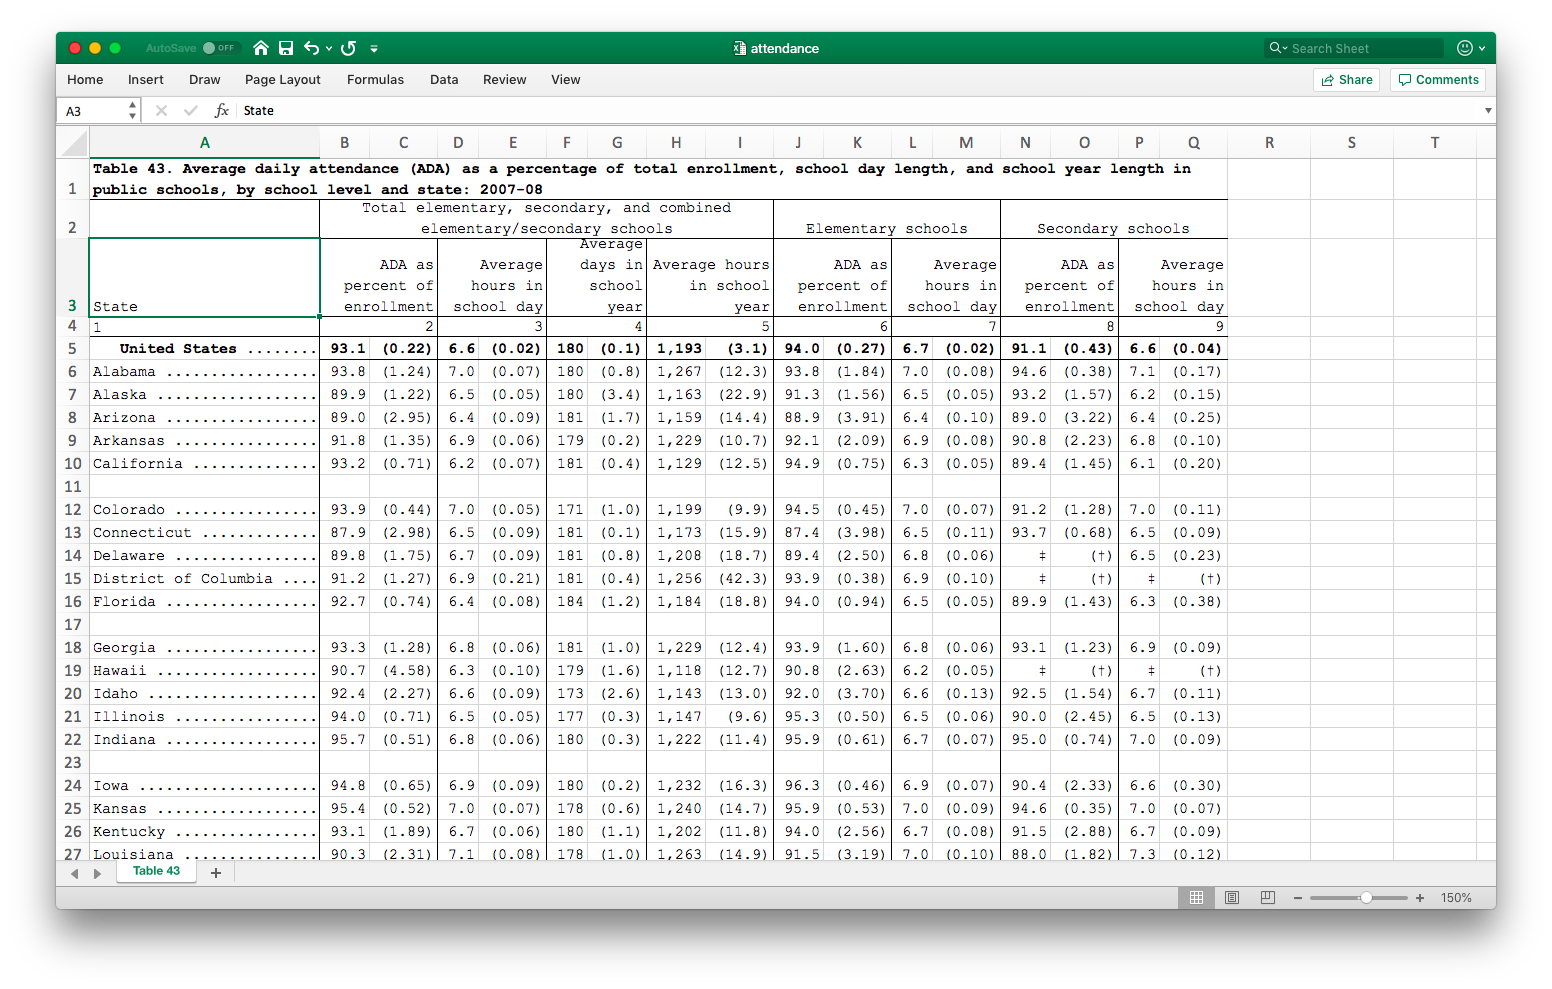
\includegraphics{img/ExcelClean.png}

Notice that there are two levels of headers on top, each spanning multiple columns.
Data is in paired columns, with the first column being the statistic and the second column
being its standard error. The first row is a title, which we don't need, and the
4th row is also not needed.

We'll first tidy-fy this dataset, and then we'll clean it up a bit. Let's first
think about the structure we want to get to for tidy-fication. The actual data lies in
the statistics and the standard errors, and each of the column groupings represents different
variables, so they should be in columns.

You can try to load this data using \texttt{import}, but you'll find it's a big mess.
There are two powerful packages (by the same group of developers), \texttt{tidyxl} and
\texttt{unpivotr}, that are fantastic tools for ``fixing'' Excel files for analysis.

Let's start with \texttt{tidyxl}.

\begin{Shaded}
\begin{Highlighting}[]
\KeywordTok{library}\NormalTok{(tidyxl)}
\end{Highlighting}
\end{Shaded}

\begin{verbatim}
## Warning: package 'tidyxl' was built under R version 3.5.2
\end{verbatim}

\begin{Shaded}
\begin{Highlighting}[]
\NormalTok{dataset1 <-}\StringTok{ }\KeywordTok{xlsx_cells}\NormalTok{(}\StringTok{'data/attendance.xlsx'}\NormalTok{)}
\NormalTok{dataset1}
\end{Highlighting}
\end{Shaded}

\begin{verbatim}
## # A tibble: 1,173 x 21
##    sheet address   row   col is_blank data_type error logical numeric
##    <chr> <chr>   <int> <int> <lgl>    <chr>     <chr> <lgl>     <dbl>
##  1 Tabl~ A1          1     1 FALSE    character <NA>  NA           NA
##  2 Tabl~ B1          1     2 TRUE     blank     <NA>  NA           NA
##  3 Tabl~ C1          1     3 TRUE     blank     <NA>  NA           NA
##  4 Tabl~ D1          1     4 TRUE     blank     <NA>  NA           NA
##  5 Tabl~ E1          1     5 TRUE     blank     <NA>  NA           NA
##  6 Tabl~ F1          1     6 TRUE     blank     <NA>  NA           NA
##  7 Tabl~ G1          1     7 TRUE     blank     <NA>  NA           NA
##  8 Tabl~ H1          1     8 TRUE     blank     <NA>  NA           NA
##  9 Tabl~ I1          1     9 TRUE     blank     <NA>  NA           NA
## 10 Tabl~ J1          1    10 TRUE     blank     <NA>  NA           NA
## # ... with 1,163 more rows, and 12 more variables: date <dttm>,
## #   character <chr>, character_formatted <list>, formula <chr>,
## #   is_array <lgl>, formula_ref <chr>, formula_group <int>, comment <chr>,
## #   height <dbl>, width <dbl>, style_format <chr>, local_format_id <int>
\end{verbatim}

Notice that this pulls in a lot of meta-data in a tidy form, including information
about cell formatting. This will be really useful in many situations.

First, lets get rid of the rows we don't need.

\begin{Shaded}
\begin{Highlighting}[]
\NormalTok{dataset1 <-}\StringTok{ }\NormalTok{dataset1 }\OperatorTok\StringTok{ }\KeywordTok{filter}\NormalTok{(row }\OperatorTok{!=}\StringTok{ }\DecValTok{1}\NormalTok{, row }\OperatorTok{!=}\StringTok{ }\DecValTok{4}\NormalTok{, row }\OperatorTok{<}\StringTok{ }\DecValTok{65}\NormalTok{)}
\end{Highlighting}
\end{Shaded}

Now we could manipulate this dataset using \texttt{tidyverse} tools, but \texttt{unpivotr} is much mor poweful.
First, we are going to pull off the two headers. \texttt{unpivotr} does this using the function \texttt{behead} (suggestive?),
with the first argument being the direction (`N', ``S'', `E',`W',etc) of the table that the header is present. We will
also consider the first column, consisting of state names, as a header on the left.

\begin{Shaded}
\begin{Highlighting}[]
\KeywordTok{library}\NormalTok{(unpivotr)}
\end{Highlighting}
\end{Shaded}

\begin{verbatim}
## Warning: package 'unpivotr' was built under R version 3.5.2
\end{verbatim}

\begin{Shaded}
\begin{Highlighting}[]
\NormalTok{dataset1 }\OperatorTok\StringTok{ }
\StringTok{  }\KeywordTok{behead}\NormalTok{(}\StringTok{'N'}\NormalTok{, tophead) }\OperatorTok\StringTok{ }
\StringTok{  }\KeywordTok{behead}\NormalTok{(}\StringTok{'N'}\NormalTok{, head2) }\OperatorTok\StringTok{ }
\StringTok{  }\KeywordTok{behead}\NormalTok{(}\StringTok{'W'}\NormalTok{, State) }\OperatorTok\StringTok{ }
\StringTok{  }\KeywordTok{select}\NormalTok{(row, col, data_type, numeric, tophead, head2, State)}
\end{Highlighting}
\end{Shaded}

\begin{verbatim}
## # A tibble: 960 x 7
##      row   col data_type  numeric tophead               head2     State    
##    <int> <int> <chr>        <dbl> <chr>                 <chr>     <chr>    
##  1     5     2 numeric    9.31e+1 Total elementary, se~ ADA as p~ "   Unit~
##  2     5     3 numeric    2.19e-1 <NA>                  <NA>      "   Unit~
##  3     5     4 numeric    6.64e+0 <NA>                  Average ~ "   Unit~
##  4     5     5 numeric    1.76e-2 <NA>                  <NA>      "   Unit~
##  5     5     6 numeric    1.80e+2 <NA>                  Average ~ "   Unit~
##  6     5     7 numeric    1.43e-1 <NA>                  <NA>      "   Unit~
##  7     5     8 numeric    1.19e+3 <NA>                  Average ~ "   Unit~
##  8     5     9 numeric    3.09e+0 <NA>                  <NA>      "   Unit~
##  9     5    10 numeric    9.40e+1 Elementary schools    ADA as p~ "   Unit~
## 10     5    11 numeric    2.69e-1 <NA>                  <NA>      "   Unit~
## # ... with 950 more rows
\end{verbatim}

We need to separate the statistics and the standard errors from consecutive columns, and
also make them headers.

\begin{Shaded}
\begin{Highlighting}[]
\NormalTok{dataset1 }\OperatorTok\StringTok{ }
\StringTok{  }\KeywordTok{behead}\NormalTok{(}\StringTok{'N'}\NormalTok{, tophead) }\OperatorTok\StringTok{ }
\StringTok{  }\KeywordTok{behead}\NormalTok{(}\StringTok{'N'}\NormalTok{, head2) }\OperatorTok\StringTok{ }
\StringTok{  }\KeywordTok{behead}\NormalTok{(}\StringTok{'W'}\NormalTok{, State) }\OperatorTok\StringTok{ }
\StringTok{  }\KeywordTok{select}\NormalTok{(row, col, data_type, numeric, tophead, head2, State) }\OperatorTok\StringTok{ }
\StringTok{  }\KeywordTok{mutate}\NormalTok{(}\DataTypeTok{header =} \KeywordTok{ifelse}\NormalTok{(col }\OperatorTok\StringTok{ }\DecValTok{2} \OperatorTok{==}\StringTok{ }\DecValTok{0}\NormalTok{, }\StringTok{'stats'}\NormalTok{,}\StringTok{'se'}\NormalTok{))}
\end{Highlighting}
\end{Shaded}

\begin{verbatim}
## # A tibble: 960 x 8
##      row   col data_type  numeric tophead          head2    State    header
##    <int> <int> <chr>        <dbl> <chr>            <chr>    <chr>    <chr> 
##  1     5     2 numeric    9.31e+1 Total elementar~ ADA as ~ "   Uni~ stats 
##  2     5     3 numeric    2.19e-1 <NA>             <NA>     "   Uni~ se    
##  3     5     4 numeric    6.64e+0 <NA>             Average~ "   Uni~ stats 
##  4     5     5 numeric    1.76e-2 <NA>             <NA>     "   Uni~ se    
##  5     5     6 numeric    1.80e+2 <NA>             Average~ "   Uni~ stats 
##  6     5     7 numeric    1.43e-1 <NA>             <NA>     "   Uni~ se    
##  7     5     8 numeric    1.19e+3 <NA>             Average~ "   Uni~ stats 
##  8     5     9 numeric    3.09e+0 <NA>             <NA>     "   Uni~ se    
##  9     5    10 numeric    9.40e+1 Elementary scho~ ADA as ~ "   Uni~ stats 
## 10     5    11 numeric    2.69e-1 <NA>             <NA>     "   Uni~ se    
## # ... with 950 more rows
\end{verbatim}

The \texttt{\%\%} operator computes the remainder if the left side is divided by the right side.
So the criterion is asking which columns are even. The \texttt{ifelse} statement says,
if the criterion is met, write ``stats'', otherwise write ``se''. This new variable
is assigned to the dataset with the variable name ``header''.

Notice that we have actually tidy-fied this dataset, but there's missing data here, since
the column headers span several rows visually but are only credited to the first column it covers.
So we need to fill in the entries for the remaining rows with the corresponding entry from the earliest column.
There is a function \texttt{fill} in \texttt{tidyr} that does this general trick, using a method called \emph{last value carried forward}.

\begin{Shaded}
\begin{Highlighting}[]
\NormalTok{dataset1 }\OperatorTok\StringTok{ }
\StringTok{  }\KeywordTok{behead}\NormalTok{(}\StringTok{'N'}\NormalTok{, tophead) }\OperatorTok\StringTok{ }
\StringTok{  }\KeywordTok{behead}\NormalTok{(}\StringTok{'N'}\NormalTok{, head2) }\OperatorTok\StringTok{ }
\StringTok{  }\KeywordTok{behead}\NormalTok{(}\StringTok{'W'}\NormalTok{, State) }\OperatorTok\StringTok{ }
\StringTok{  }\KeywordTok{select}\NormalTok{(row, col, data_type, numeric, tophead, head2, State) }\OperatorTok\StringTok{ }
\StringTok{  }\KeywordTok{fill}\NormalTok{(tophead) }\OperatorTok\StringTok{ }
\StringTok{  }\KeywordTok{fill}\NormalTok{(head2)}
\end{Highlighting}
\end{Shaded}

\begin{verbatim}
## # A tibble: 960 x 7
##      row   col data_type  numeric tophead               head2     State    
##    <int> <int> <chr>        <dbl> <chr>                 <chr>     <chr>    
##  1     5     2 numeric    9.31e+1 Total elementary, se~ ADA as p~ "   Unit~
##  2     5     3 numeric    2.19e-1 Total elementary, se~ ADA as p~ "   Unit~
##  3     5     4 numeric    6.64e+0 Total elementary, se~ Average ~ "   Unit~
##  4     5     5 numeric    1.76e-2 Total elementary, se~ Average ~ "   Unit~
##  5     5     6 numeric    1.80e+2 Total elementary, se~ Average ~ "   Unit~
##  6     5     7 numeric    1.43e-1 Total elementary, se~ Average ~ "   Unit~
##  7     5     8 numeric    1.19e+3 Total elementary, se~ Average ~ "   Unit~
##  8     5     9 numeric    3.09e+0 Total elementary, se~ Average ~ "   Unit~
##  9     5    10 numeric    9.40e+1 Elementary schools    ADA as p~ "   Unit~
## 10     5    11 numeric    2.69e-1 Elementary schools    ADA as p~ "   Unit~
## # ... with 950 more rows
\end{verbatim}

To make this really tidy, we need to make two columns titled \texttt{stats} and \texttt{se} from this.
We've seen this using \texttt{spread}, but there is a slightly more robust method from \texttt{unpivotr} called
\texttt{spatter} which is meant for this unique structure.

\begin{Shaded}
\begin{Highlighting}[]
\NormalTok{tidy_dataset <-}\StringTok{ }\NormalTok{dataset1 }\OperatorTok\StringTok{ }
\StringTok{  }\KeywordTok{behead}\NormalTok{(}\StringTok{'N'}\NormalTok{, tophead) }\OperatorTok\StringTok{ }
\StringTok{  }\KeywordTok{behead}\NormalTok{(}\StringTok{'N'}\NormalTok{, head2) }\OperatorTok\StringTok{ }
\StringTok{  }\KeywordTok{behead}\NormalTok{(}\StringTok{'W'}\NormalTok{, State) }\OperatorTok\StringTok{ }
\StringTok{  }\KeywordTok{select}\NormalTok{(row, col, data_type, numeric, tophead, head2, State) }\OperatorTok\StringTok{ }
\StringTok{  }\KeywordTok{mutate}\NormalTok{(}\DataTypeTok{header =} \KeywordTok{ifelse}\NormalTok{(col }\OperatorTok\StringTok{ }\DecValTok{2} \OperatorTok{==}\StringTok{ }\DecValTok{0}\NormalTok{, }\StringTok{'stats'}\NormalTok{,}\StringTok{'se'}\NormalTok{)) }\OperatorTok\StringTok{ }
\StringTok{  }\KeywordTok{fill}\NormalTok{(tophead) }\OperatorTok\StringTok{ }
\StringTok{  }\KeywordTok{fill}\NormalTok{(head2) }\OperatorTok\StringTok{ }
\StringTok{  }\KeywordTok{select}\NormalTok{(row, numeric, tophead, head2, State, header) }\OperatorTok\StringTok{ }
\StringTok{  }\KeywordTok{spatter}\NormalTok{(header, numeric) }\OperatorTok\StringTok{ }
\StringTok{  }\KeywordTok{select}\NormalTok{(}\OperatorTok{-}\NormalTok{row)}
\NormalTok{tidy_dataset}
\end{Highlighting}
\end{Shaded}

\begin{verbatim}
## # A tibble: 480 x 5
##    tophead                        head2          State            se  stats
##    <chr>                          <chr>          <chr>         <dbl>  <dbl>
##  1 Elementary schools             ADA as percen~ "   United ~ 0.269  9.40e1
##  2 Elementary schools             Average hours~ "   United ~ 0.0160 6.66e0
##  3 Secondary schools              ADA as percen~ "   United ~ 0.432  9.11e1
##  4 Secondary schools              Average hours~ "   United ~ 0.0403 6.59e0
##  5 Total elementary, secondary, ~ ADA as percen~ "   United ~ 0.219  9.31e1
##  6 Total elementary, secondary, ~ Average days ~ "   United ~ 0.143  1.80e2
##  7 Total elementary, secondary, ~ Average hours~ "   United ~ 0.0176 6.64e0
##  8 Total elementary, secondary, ~ Average hours~ "   United ~ 3.09   1.19e3
##  9 Elementary schools             ADA as percen~ Alabama ...~ 1.84   9.38e1
## 10 Elementary schools             Average hours~ Alabama ...~ 0.0759 7.04e0
## # ... with 470 more rows
\end{verbatim}

We have to clean the \texttt{State} variable. We'll use the methods in the \texttt{stringr}
package, which is already loaded with the \texttt{tidyverse}.

\begin{Shaded}
\begin{Highlighting}[]
\NormalTok{tidy_dataset <-}\StringTok{ }\NormalTok{tidy_dataset }\OperatorTok\StringTok{ }
\StringTok{  }\KeywordTok{mutate}\NormalTok{(}\DataTypeTok{State =} \KeywordTok{str_remove}\NormalTok{(State, }\StringTok{'}\CharTok{\textbackslash{}\textbackslash{}}\StringTok{.+'}\NormalTok{)) }\OperatorTok\StringTok{ }
\StringTok{  }\KeywordTok{mutate}\NormalTok{(}\DataTypeTok{State =} \KeywordTok{str_trim}\NormalTok{(State))}
\end{Highlighting}
\end{Shaded}

The first verb removes all the \texttt{.} in the variable, using something called a regular expression.
This particular expression means that we want to look for sequences of dots, and remove them.
The \texttt{\textbackslash{}\textbackslash{}} before the \texttt{.} tells R that we really mean \texttt{.}, since the \texttt{.} has a different meaning in
regular expressions.

The second verb trims away blank spaces before and after each entry.

We'll hold on to this dataset for the visualization section. Just to be safe, let's
save it.

\begin{Shaded}
\begin{Highlighting}[]
\KeywordTok{saveRDS}\NormalTok{(tidy_dataset, }\DataTypeTok{file =} \StringTok{'data/attendance.rds'}\NormalTok{)}
\end{Highlighting}
\end{Shaded}

This saves the data in an R-specific format that will allow us to load it quickly.

\begin{quote}
The RDS format is an open standard and so it can be called from other programs if the
appropriate programs are written.
\end{quote}

\hypertarget{dealing-with-visual-formating-colors}{%
\subsection*{Dealing with visual formating (colors)}\label{dealing-with-visual-formating-colors}}
\addcontentsline{toc}{subsection}{Dealing with visual formating (colors)}

The dataset we'll use for this has identifiable information, so I will not expose
it publicly. It is available in your files as \texttt{data/classlist.xlsx}.

Since we're interested in background and font colors here, which are informative,
we also need to load the format information into R.

\begin{Shaded}
\begin{Highlighting}[]
\KeywordTok{library}\NormalTok{(tidyxl)}
\KeywordTok{library}\NormalTok{(unpivotr)}

\NormalTok{dataset2 <-}\StringTok{ }\KeywordTok{xlsx_cells}\NormalTok{(}\StringTok{'data/classlist.xlsx'}\NormalTok{)}
\NormalTok{formats <-}\StringTok{ }\KeywordTok{xlsx_formats}\NormalTok{(}\StringTok{'data/classlist.xlsx'}\NormalTok{)}

\NormalTok{format_id <-}\StringTok{ }\NormalTok{dataset2}\OperatorTok{$}\NormalTok{local_format_id}
\NormalTok{dataset2}\OperatorTok{$}\NormalTok{font_color <-}\StringTok{ }\NormalTok{formats}\OperatorTok{$}\NormalTok{local}\OperatorTok{$}\NormalTok{font}\OperatorTok{$}\NormalTok{color}\OperatorTok{$}\NormalTok{rgb[format_id]}
\NormalTok{dataset2}\OperatorTok{$}\NormalTok{bg_color <-}\StringTok{ }\NormalTok{formats}\OperatorTok{$}\NormalTok{local}\OperatorTok{$}\NormalTok{fill}\OperatorTok{$}\NormalTok{patternFill}\OperatorTok{$}\NormalTok{fgColor}\OperatorTok{$}\NormalTok{rgb[format_id]}
\end{Highlighting}
\end{Shaded}

\begin{Shaded}
\begin{Highlighting}[]
\KeywordTok{unique}\NormalTok{(dataset2}\OperatorTok{$}\NormalTok{font_color)}
\end{Highlighting}
\end{Shaded}

\begin{verbatim}
## [1] "FF000000" "FF0563C1" "FFFF0000"
\end{verbatim}

\begin{Shaded}
\begin{Highlighting}[]
\KeywordTok{unique}\NormalTok{(dataset2}\OperatorTok{$}\NormalTok{bg_color)}
\end{Highlighting}
\end{Shaded}

\begin{verbatim}
## [1] "FFFFC000" NA         "FFE7E6E6"
\end{verbatim}

So we can filter rows based on these two colors if we want.

To tidy-fy this dataset, we realize that there are really two interweaved datasets.
The odd rows are one dataset and the even rows are another dataset.

\begin{Shaded}
\begin{Highlighting}[]
\NormalTok{dat1 <-}\StringTok{ }\NormalTok{dataset2 }\OperatorTok\StringTok{ }
\StringTok{  }\KeywordTok{filter}\NormalTok{( row }\OperatorTok\StringTok{ }\DecValTok{2} \OperatorTok{==}\StringTok{ }\DecValTok{1}\NormalTok{) }\OperatorTok\StringTok{ }\CommentTok{# odd rows}
\StringTok{  }\KeywordTok{behead}\NormalTok{(}\StringTok{'N'}\NormalTok{, header) }\OperatorTok\StringTok{ }
\StringTok{  }\KeywordTok{mutate}\NormalTok{(}\DataTypeTok{row =}\NormalTok{ (row}\OperatorTok{+}\DecValTok{1}\NormalTok{)}\OperatorTok{/}\DecValTok{2}\NormalTok{) }\CommentTok{# make the row numbers sequential}

\NormalTok{dat2 <-}\StringTok{ }\NormalTok{dataset2 }\OperatorTok\StringTok{ }
\StringTok{  }\KeywordTok{filter}\NormalTok{(row }\OperatorTok\StringTok{ }\DecValTok{2} \OperatorTok{==}\StringTok{ }\DecValTok{0}\NormalTok{) }\OperatorTok\StringTok{  }\CommentTok{# even rows}
\StringTok{  }\KeywordTok{behead}\NormalTok{(}\StringTok{'N'}\NormalTok{, header) }\OperatorTok\StringTok{ }
\StringTok{  }\KeywordTok{mutate}\NormalTok{(}\DataTypeTok{row =}\NormalTok{ row}\OperatorTok{/}\DecValTok{2}\NormalTok{) }\OperatorTok\StringTok{ }\CommentTok{# make row numbers sequential}
\StringTok{  }\KeywordTok{mutate}\NormalTok{(}\DataTypeTok{col =}\NormalTok{ col}\OperatorTok{+}\DecValTok{4}\NormalTok{) }\CommentTok{# These will be the last 4 cols of new data}

\NormalTok{tidy_dataset2 <-}\StringTok{ }
\StringTok{  }\KeywordTok{rbind}\NormalTok{(dat1, dat2) }\OperatorTok\StringTok{ }\CommentTok{# Put datsets on top of each other}
\StringTok{  }\KeywordTok{select}\NormalTok{(row, data_type, numeric, character, header) }\OperatorTok\StringTok{ }
\StringTok{  }\KeywordTok{spatter}\NormalTok{(header) }\OperatorTok\StringTok{ }
\StringTok{  }\KeywordTok{select}\NormalTok{(}\OperatorTok{-}\NormalTok{row, }\OperatorTok{-}\NormalTok{numeric)}
\end{Highlighting}
\end{Shaded}

We'll do a couple of finesse things to finish. First, we'll make the names with
no spaces (they're a pain to write otherwise) and put the student name on
the first column.

\begin{Shaded}
\begin{Highlighting}[]
\NormalTok{tidy_dataset2 <-}\StringTok{ }\NormalTok{tidy_dataset2 }\OperatorTok\StringTok{ }
\StringTok{  }\KeywordTok{set_names}\NormalTok{(}\KeywordTok{make.names}\NormalTok{(}\KeywordTok{names}\NormalTok{(.))) }\OperatorTok\StringTok{ }
\StringTok{  }\KeywordTok{select}\NormalTok{(Student.Name, }\KeywordTok{everything}\NormalTok{())}
\end{Highlighting}
\end{Shaded}

\texttt{make.names} changes a vector of names into ``approved'' space-free format, replacing
the space with \texttt{.}. One shortcut I've used is using \texttt{.} as an argument to \texttt{names}, which
means that the \texttt{.} is replaced by the ``noun'' that is being acted on by the ``verbs''. You will
notice that I can also do multiple verbs together to work sequentially.

\hypertarget{sec:description}{%
\chapter{Describing data}\label{sec:description}}

Data cleaning and munging is important, yet tedious work. Now that we're done
with that, we can get to the fun part of exploring the data.

Our workhorse for this will be the \texttt{dplyr} package, part of the \texttt{tidyverse}. This
package provides 5 basic verbs:

\begin{itemize}
\tightlist
\item
  \texttt{filter}: filter a dataset by rows
\item
  \texttt{select}: select columns of a dataset
\item
  \texttt{arrange}: arrange rows of a dataset by values of some variables
\item
  \texttt{group\_by}: split a dataset by values of some variables, so that we can apply verbs to each split
\item
  \texttt{summarize}: compute various summaries from the data
\end{itemize}

\texttt{dplyr} also has verbs to let stitch datasets together, which are \texttt{left\_join},
\texttt{right\_join}, \texttt{inner\_join}, \texttt{outer\_join}, \texttt{semi\_join}, \texttt{anti\_join}, \texttt{bind\_rows} and
\texttt{bind\_cols}.

I'll be using the latest \texttt{dplyr}, version 0.8.0.9009. If you have
an older version, most but not all things will work.

We'll start with the in-build \texttt{mtcars} dataset.

\begin{Shaded}
\begin{Highlighting}[]
\KeywordTok{library}\NormalTok{(tidyverse)}
\NormalTok{mtcars1 <-}\StringTok{ }\NormalTok{mtcars }\OperatorTok\StringTok{ }\KeywordTok{rownames_to_column}\NormalTok{(}\StringTok{'cars'}\NormalTok{) }\OperatorTok\StringTok{ }\KeywordTok{as_tibble}\NormalTok{()}
\NormalTok{mtcars1}
\end{Highlighting}
\end{Shaded}

\begin{verbatim}
## # A tibble: 32 x 12
##    cars     mpg   cyl  disp    hp  drat    wt  qsec    vs    am  gear  carb
##    <chr>  <dbl> <dbl> <dbl> <dbl> <dbl> <dbl> <dbl> <dbl> <dbl> <dbl> <dbl>
##  1 Mazda~  21       6  160    110  3.9   2.62  16.5     0     1     4     4
##  2 Mazda~  21       6  160    110  3.9   2.88  17.0     0     1     4     4
##  3 Datsu~  22.8     4  108     93  3.85  2.32  18.6     1     1     4     1
##  4 Horne~  21.4     6  258    110  3.08  3.22  19.4     1     0     3     1
##  5 Horne~  18.7     8  360    175  3.15  3.44  17.0     0     0     3     2
##  6 Valia~  18.1     6  225    105  2.76  3.46  20.2     1     0     3     1
##  7 Duste~  14.3     8  360    245  3.21  3.57  15.8     0     0     3     4
##  8 Merc ~  24.4     4  147.    62  3.69  3.19  20       1     0     4     2
##  9 Merc ~  22.8     4  141.    95  3.92  3.15  22.9     1     0     4     2
## 10 Merc ~  19.2     6  168.   123  3.92  3.44  18.3     1     0     4     4
## # ... with 22 more rows
\end{verbatim}

Let's get some summary statistics from this dataset. First, let's compute the average
mpg, displacement, and horsepower of these cars.

\begin{Shaded}
\begin{Highlighting}[]
\NormalTok{mtcars1 }\OperatorTok\StringTok{ }\KeywordTok{summarize}\NormalTok{(}\DataTypeTok{mpg =} \KeywordTok{mean}\NormalTok{(mpg, }\DataTypeTok{na.rm=}\NormalTok{T), }\DataTypeTok{disp =} \KeywordTok{mean}\NormalTok{(disp, }\DataTypeTok{na.rm=}\NormalTok{T), }\DataTypeTok{hp =} \KeywordTok{mean}\NormalTok{(hp, }\DataTypeTok{na.rm=}\NormalTok{T))}
\end{Highlighting}
\end{Shaded}

\begin{verbatim}
## # A tibble: 1 x 3
##     mpg  disp    hp
##   <dbl> <dbl> <dbl>
## 1  20.1  231.  147.
\end{verbatim}

\begin{quote}
I'm adding the option \texttt{na.rm=T} to remove any missing values; if there is even a single missing value, the mean will be computed as \texttt{NA}
\end{quote}

Most \texttt{dplyr} verbs also have scoped versions \texttt{*\_all}, \texttt{*\_at}, \texttt{*\_if}, which can be useful. The \texttt{*\_any} versions act
upon all the columns, the \texttt{*\_at} versions on specified columns (same way columns are specified in \texttt{select}) and the
\texttt{*\_if} versions on columns with particular properties. So the above code could be written as

\begin{Shaded}
\begin{Highlighting}[]
\NormalTok{mtcars1 }\OperatorTok\StringTok{ }\KeywordTok{summarize_at}\NormalTok{(}\KeywordTok{vars}\NormalTok{(mpg, disp, hp), mean, }\DataTypeTok{na.rm =}\NormalTok{ T)}
\end{Highlighting}
\end{Shaded}

\begin{verbatim}
## # A tibble: 1 x 3
##     mpg  disp    hp
##   <dbl> <dbl> <dbl>
## 1  20.1  231.  147.
\end{verbatim}

\hypertarget{factors-or-categorical-variables}{%
\subsection*{Factors or categorical variables}\label{factors-or-categorical-variables}}
\addcontentsline{toc}{subsection}{Factors or categorical variables}

R has a data type called a \texttt{factor}, which is meant for categorical or discrete variables; things like sex, race, and,
in this data, \texttt{cyl}. We need to transform the column to this data type first.

\begin{Shaded}
\begin{Highlighting}[]
\NormalTok{mtcars1 <-}\StringTok{ }\NormalTok{mtcars1 }\OperatorTok\StringTok{ }
\StringTok{  }\KeywordTok{mutate}\NormalTok{(}\DataTypeTok{cyl =} \KeywordTok{as.factor}\NormalTok{(cyl))}
\end{Highlighting}
\end{Shaded}

There are a few others that might need this treatment.

\begin{Shaded}
\begin{Highlighting}[]
\NormalTok{mtcars1 <-}\StringTok{ }\NormalTok{mtcars1 }\OperatorTok\StringTok{ }
\StringTok{  }\KeywordTok{mutate_at}\NormalTok{(}\KeywordTok{vars}\NormalTok{(cyl, vs, am, gear, carb), as.factor)}
\end{Highlighting}
\end{Shaded}

Let's see what we've done.

\begin{Shaded}
\begin{Highlighting}[]
\KeywordTok{str}\NormalTok{(mtcars1)}
\end{Highlighting}
\end{Shaded}

\begin{verbatim}
## Classes 'tbl_df', 'tbl' and 'data.frame':    32 obs. of  12 variables:
##  $ cars: chr  "Mazda RX4" "Mazda RX4 Wag" "Datsun 710" "Hornet 4 Drive" ...
##  $ mpg : num  21 21 22.8 21.4 18.7 18.1 14.3 24.4 22.8 19.2 ...
##  $ cyl : Factor w/ 3 levels "4","6","8": 2 2 1 2 3 2 3 1 1 2 ...
##  $ disp: num  160 160 108 258 360 ...
##  $ hp  : num  110 110 93 110 175 105 245 62 95 123 ...
##  $ drat: num  3.9 3.9 3.85 3.08 3.15 2.76 3.21 3.69 3.92 3.92 ...
##  $ wt  : num  2.62 2.88 2.32 3.21 3.44 ...
##  $ qsec: num  16.5 17 18.6 19.4 17 ...
##  $ vs  : Factor w/ 2 levels "0","1": 1 1 2 2 1 2 1 2 2 2 ...
##  $ am  : Factor w/ 2 levels "0","1": 2 2 2 1 1 1 1 1 1 1 ...
##  $ gear: Factor w/ 3 levels "3","4","5": 2 2 2 1 1 1 1 2 2 2 ...
##  $ carb: Factor w/ 6 levels "1","2","3","4",..: 4 4 1 1 2 1 4 2 2 4 ...
\end{verbatim}

Now, let's compute averages of all the non-factor, or numeric, variables.

\begin{Shaded}
\begin{Highlighting}[]
\NormalTok{mtcars1 }\OperatorTok\StringTok{ }\KeywordTok{summarize_if}\NormalTok{(is.numeric, mean)}
\end{Highlighting}
\end{Shaded}

\begin{verbatim}
## # A tibble: 1 x 6
##     mpg  disp    hp  drat    wt  qsec
##   <dbl> <dbl> <dbl> <dbl> <dbl> <dbl>
## 1  20.1  231.  147.  3.60  3.22  17.8
\end{verbatim}

We can get a summary of all the variables using the function \texttt{summary}.

\begin{Shaded}
\begin{Highlighting}[]
\KeywordTok{summary}\NormalTok{(mtcars1)}
\end{Highlighting}
\end{Shaded}

\begin{verbatim}
##      cars                mpg        cyl         disp             hp       
##  Length:32          Min.   :10.40   4:11   Min.   : 71.1   Min.   : 52.0  
##  Class :character   1st Qu.:15.43   6: 7   1st Qu.:120.8   1st Qu.: 96.5  
##  Mode  :character   Median :19.20   8:14   Median :196.3   Median :123.0  
##                     Mean   :20.09          Mean   :230.7   Mean   :146.7  
##                     3rd Qu.:22.80          3rd Qu.:326.0   3rd Qu.:180.0  
##                     Max.   :33.90          Max.   :472.0   Max.   :335.0  
##       drat             wt             qsec       vs     am     gear  
##  Min.   :2.760   Min.   :1.513   Min.   :14.50   0:18   0:19   3:15  
##  1st Qu.:3.080   1st Qu.:2.581   1st Qu.:16.89   1:14   1:13   4:12  
##  Median :3.695   Median :3.325   Median :17.71                 5: 5  
##  Mean   :3.597   Mean   :3.217   Mean   :17.85                       
##  3rd Qu.:3.920   3rd Qu.:3.610   3rd Qu.:18.90                       
##  Max.   :4.930   Max.   :5.424   Max.   :22.90                       
##  carb  
##  1: 7  
##  2:10  
##  3: 3  
##  4:10  
##  6: 1  
##  8: 1
\end{verbatim}

However, this does not give us a tidy dataset. Some alternatives are the \texttt{skimr} package and
the \texttt{ezsummary} package.

\begin{Shaded}
\begin{Highlighting}[]
\CommentTok{# install.packages('skimr')}
\KeywordTok{library}\NormalTok{(skimr)}
\end{Highlighting}
\end{Shaded}

\begin{verbatim}
## Warning: package 'skimr' was built under R version 3.5.2
\end{verbatim}

\begin{verbatim}
## 
## Attaching package: 'skimr'
\end{verbatim}

\begin{verbatim}
## The following object is masked from 'package:stats':
## 
##     filter
\end{verbatim}

\begin{Shaded}
\begin{Highlighting}[]
\KeywordTok{skim}\NormalTok{(mtcars1)}
\end{Highlighting}
\end{Shaded}

\begin{verbatim}
## Skim summary statistics
##  n obs: 32 
##  n variables: 12 
## 
## -- Variable type:character -----------------------------------------------------------------------------------------------
##  variable missing complete  n min max empty n_unique
##      cars       0       32 32   7  19     0       32
## 
## -- Variable type:factor --------------------------------------------------------------------------------------------------
##  variable missing complete  n n_unique                top_counts ordered
##        am       0       32 32        2       0: 19, 1: 13, NA: 0   FALSE
##      carb       0       32 32        6  2: 10, 4: 10, 1: 7, 3: 3   FALSE
##       cyl       0       32 32        3 8: 14, 4: 11, 6: 7, NA: 0   FALSE
##      gear       0       32 32        3 3: 15, 4: 12, 5: 5, NA: 0   FALSE
##        vs       0       32 32        2       0: 18, 1: 14, NA: 0   FALSE
## 
## -- Variable type:numeric -------------------------------------------------------------------------------------------------
##  variable missing complete  n   mean     sd    p0    p25    p50    p75
##      disp       0       32 32 230.72 123.94 71.1  120.83 196.3  326   
##      drat       0       32 32   3.6    0.53  2.76   3.08   3.7    3.92
##        hp       0       32 32 146.69  68.56 52     96.5  123    180   
##       mpg       0       32 32  20.09   6.03 10.4   15.43  19.2   22.8 
##      qsec       0       32 32  17.85   1.79 14.5   16.89  17.71  18.9 
##        wt       0       32 32   3.22   0.98  1.51   2.58   3.33   3.61
##    p100     hist
##  472    ▇▆▁▂▅▃▁▂
##    4.93 ▃▇▁▅▇▂▁▁
##  335    ▃▇▃▅▂▃▁▁
##   33.9  ▃▇▇▇▃▂▂▂
##   22.9  ▃▂▇▆▃▃▁▁
##    5.42 ▃▃▃▇▆▁▁▂
\end{verbatim}

\hypertarget{split-apply-combine-a.k.a.-mapreduce}{%
\section{Split-apply-combine, a.k.a. MapReduce}\label{split-apply-combine-a.k.a.-mapreduce}}

The split-apply-combine is a powerful paradigm for understanding subgroups within a dataset. The basic
idea is that you split the data into pieces based on values of some variables, do something (the same thing) to
each piece, and then stitch the results back together.

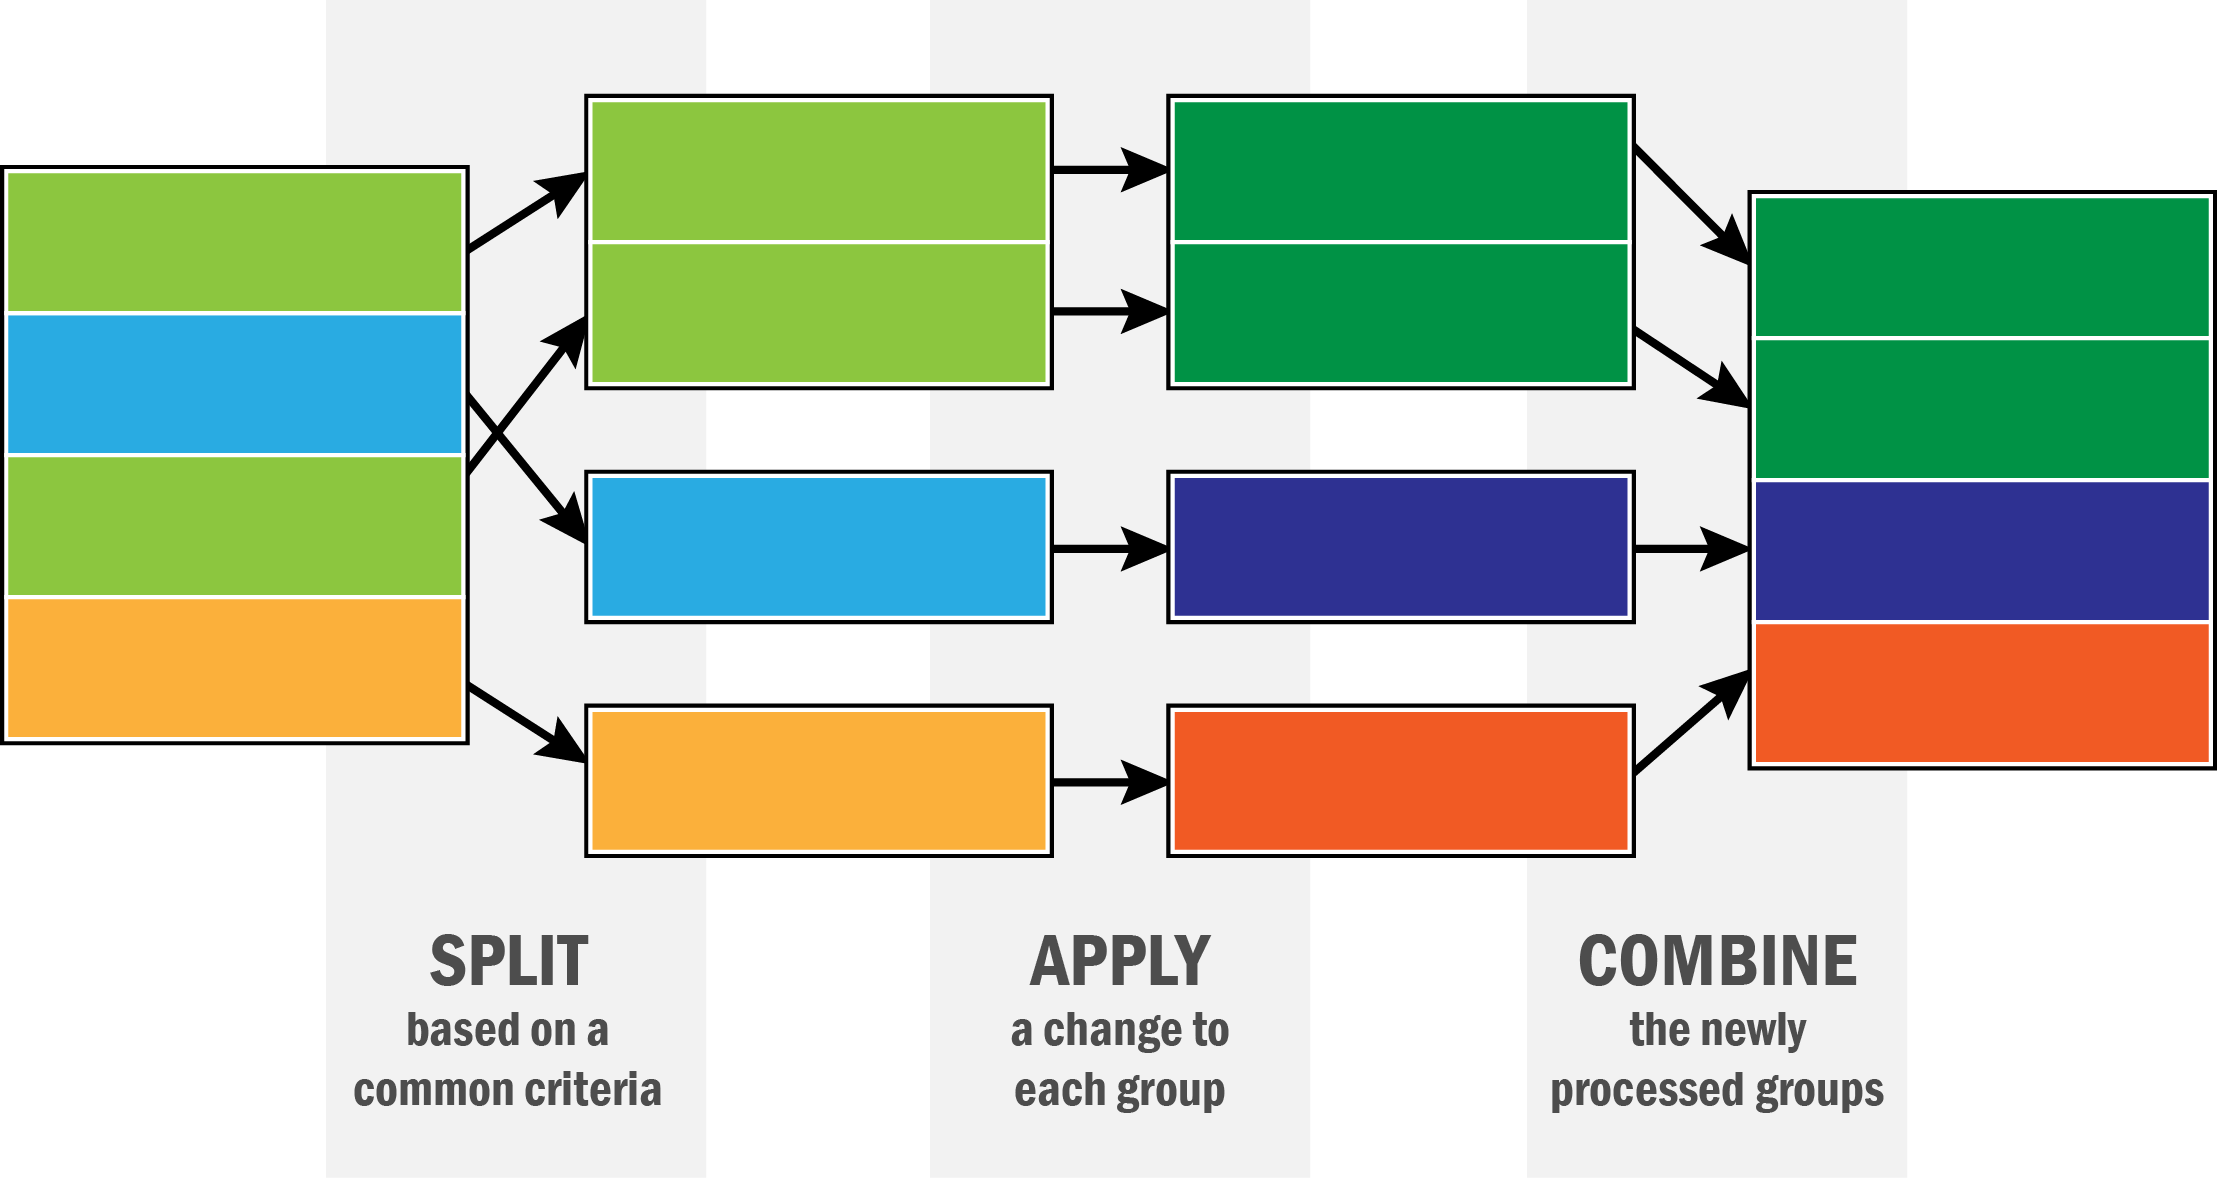
\includegraphics{img/split-apply-combine.png}

For example, in the mtcars data, we might want to know what the average mpg is by the number of cylinders. The
way to do this is:

\begin{Shaded}
\begin{Highlighting}[]
\NormalTok{mtcars1 }\OperatorTok\StringTok{ }
\StringTok{  }\KeywordTok{group_by}\NormalTok{(cyl) }\OperatorTok\StringTok{ }
\StringTok{  }\KeywordTok{summarize}\NormalTok{(}\DataTypeTok{mpg_mean =} \KeywordTok{mean}\NormalTok{(mpg))}
\end{Highlighting}
\end{Shaded}

\begin{verbatim}
## # A tibble: 3 x 2
##   cyl   mpg_mean
##   <fct>    <dbl>
## 1 4         26.7
## 2 6         19.7
## 3 8         15.1
\end{verbatim}

Once again, the scoped versions of \texttt{summarize} will also work in this pipe

\begin{Shaded}
\begin{Highlighting}[]
\NormalTok{mtcars1 }\OperatorTok\StringTok{ }
\StringTok{  }\KeywordTok{group_by}\NormalTok{(cyl) }\OperatorTok\StringTok{ }
\StringTok{  }\KeywordTok{summarize_if}\NormalTok{(is.numeric, mean)}
\end{Highlighting}
\end{Shaded}

\begin{verbatim}
## # A tibble: 3 x 7
##   cyl     mpg  disp    hp  drat    wt  qsec
##   <fct> <dbl> <dbl> <dbl> <dbl> <dbl> <dbl>
## 1 4      26.7  105.  82.6  4.07  2.29  19.1
## 2 6      19.7  183. 122.   3.59  3.12  18.0
## 3 8      15.1  353. 209.   3.23  4.00  16.8
\end{verbatim}

Let's go a bit further and compute the medians as well.

\begin{Shaded}
\begin{Highlighting}[]
\NormalTok{mtcars1 }\OperatorTok\StringTok{ }
\StringTok{  }\KeywordTok{group_by}\NormalTok{(cyl) }\OperatorTok\StringTok{ }
\StringTok{  }\KeywordTok{summarize_if}\NormalTok{(is.numeric, }\KeywordTok{list}\NormalTok{(}\StringTok{'mean'}\NormalTok{=}\StringTok{ }\NormalTok{mean, }\StringTok{'median'}\NormalTok{ =}\StringTok{ }\NormalTok{median))}
\end{Highlighting}
\end{Shaded}

\begin{verbatim}
## # A tibble: 3 x 13
##   cyl   mpg_mean disp_mean hp_mean drat_mean wt_mean qsec_mean mpg_median
##   <fct>    <dbl>     <dbl>   <dbl>     <dbl>   <dbl>     <dbl>      <dbl>
## 1 4         26.7      105.    82.6      4.07    2.29      19.1       26  
## 2 6         19.7      183.   122.       3.59    3.12      18.0       19.7
## 3 8         15.1      353.   209.       3.23    4.00      16.8       15.2
## # ... with 5 more variables: disp_median <dbl>, hp_median <dbl>,
## #   drat_median <dbl>, wt_median <dbl>, qsec_median <dbl>
\end{verbatim}

We can look at a second dataset showing individual violent incidents in Western Afrika
between 2000 and 2017. We can get the number of incidents per country and year very easily using this paradigm.

\begin{Shaded}
\begin{Highlighting}[]
\NormalTok{west_africa <-}\StringTok{ }\KeywordTok{import}\NormalTok{(}\StringTok{'data/2000-01-01-2019-01-01-Western_Africa.csv'}\NormalTok{)}
\NormalTok{west_africa }\OperatorTok\StringTok{ }\KeywordTok{group_by}\NormalTok{(country, year) }\OperatorTok\StringTok{ }\KeywordTok{tally}\NormalTok{()}
\end{Highlighting}
\end{Shaded}

\begin{verbatim}
## # A tibble: 290 x 3
## # Groups:   country [15]
##    country  year     n
##    <chr>   <int> <int>
##  1 Benin    2000     1
##  2 Benin    2001     3
##  3 Benin    2002     1
##  4 Benin    2003     2
##  5 Benin    2004     2
##  6 Benin    2005     2
##  7 Benin    2006     1
##  8 Benin    2007     3
##  9 Benin    2008     1
## 10 Benin    2009     2
## # ... with 280 more rows
\end{verbatim}

For display, we can make this a wide dataset

\begin{Shaded}
\begin{Highlighting}[]
\NormalTok{west_africa }\OperatorTok\StringTok{ }\KeywordTok{group_by}\NormalTok{(country, year) }\OperatorTok\StringTok{ }\KeywordTok{tally}\NormalTok{() }\OperatorTok\StringTok{ }
\StringTok{  }\KeywordTok{spread}\NormalTok{(year, n)}
\end{Highlighting}
\end{Shaded}

\begin{verbatim}
## # A tibble: 15 x 21
## # Groups:   country [15]
##    country `2000` `2001` `2002` `2003` `2004` `2005` `2006` `2007` `2008`
##    <chr>    <int>  <int>  <int>  <int>  <int>  <int>  <int>  <int>  <int>
##  1 Benin        1      3      1      2      2      2      1      3      1
##  2 Burkin~     22      6      6      1      4      6      8      1     12
##  3 Gambia       8     14     13     11      5      4      6      2      4
##  4 Ghana       10      8      7     17      7      3      3      5     11
##  5 Guinea     180     70     14     10     11     15      7     46     15
##  6 Guinea~      9      2      3      5      4     13     21      2      2
##  7 Ivory ~    133     34    135    177    101     45     30      6     24
##  8 Liberia     87    171    148    242     22     26     22      9     17
##  9 Mali         4      5      2      3      3      2     10     11     21
## 10 Maurit~      4      1      3     13      2      9      3      5     16
## 11 Niger       11      9     42      6     17      9      8     31     28
## 12 Nigeria    168    118    160    207    277    198    120    200    208
## 13 Senegal     86     61     40     18     11     11     29     24     20
## 14 Sierra~    495    224      5     18     14      5      1      6     15
## 15 Togo         4      4      3      4      3     25      1      1      1
## # ... with 11 more variables: `2009` <int>, `2010` <int>, `2011` <int>,
## #   `2012` <int>, `2013` <int>, `2014` <int>, `2015` <int>, `2016` <int>,
## #   `2017` <int>, `2018` <int>, `2019` <int>
\end{verbatim}

We'll save this dataset for visualization later.

\begin{Shaded}
\begin{Highlighting}[]
\NormalTok{west_africa }\OperatorTok\StringTok{ }\KeywordTok{group_by}\NormalTok{(country, year) }\OperatorTok\StringTok{ }\KeywordTok{tally}\NormalTok{() }\OperatorTok\StringTok{ }
\StringTok{  }\KeywordTok{spread}\NormalTok{(year, n) }\OperatorTok\StringTok{ }
\StringTok{  }\KeywordTok{saveRDS}\NormalTok{(}\StringTok{'data/west_africa.rds'}\NormalTok{)}
\end{Highlighting}
\end{Shaded}

\hypertarget{joins}{%
\section{Joins}\label{joins}}

We mentioned earlier that there are several kinds of ways we can join data. The
different kinds of joins are described below.

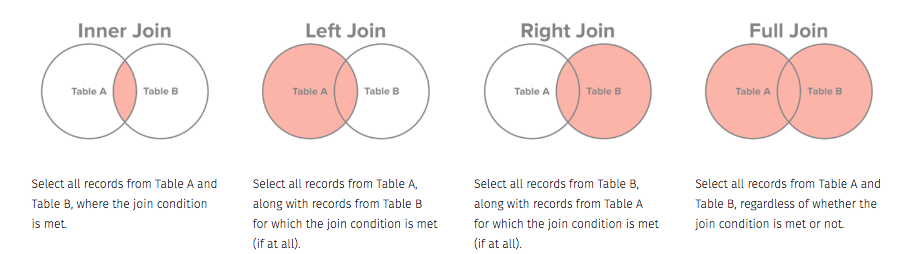
\includegraphics{img/joins.png}

Let's look at these joins with an example. We have two simulated datasets looking at
DOS real estate allocation and staffing. We will look at how much area on average each
bureau has given the number of employees

\begin{Shaded}
\begin{Highlighting}[]
\NormalTok{staffing_data <-}\StringTok{ }\KeywordTok{import}\NormalTok{(}\StringTok{'data/Staffing_by_Bureau.csv'}\NormalTok{) }\OperatorTok\StringTok{ }\KeywordTok{as_tibble}\NormalTok{()}
\NormalTok{real_estate <-}\StringTok{ }\KeywordTok{import}\NormalTok{(}\StringTok{'data/DoS_Real_Estate_Allocation.csv'}\NormalTok{) }\OperatorTok\StringTok{ }\KeywordTok{as_tibble}\NormalTok{()}
\NormalTok{real_estate}
\end{Highlighting}
\end{Shaded}

\begin{verbatim}
## # A tibble: 666 x 4
##    Building Bureau               Location  Size
##    <chr>    <chr>                   <int> <int>
##  1 HST      Administration (A)       4779   640
##  2 SA2      Administration (A)       4801  1090
##  3 HST      Administration (A)       5109  1040
##  4 HST      Administration (A)       3717  1620
##  5 SA4      Administration (A)       3940  1390
##  6 HST      Administration (A)       3661  1480
##  7 HST      Administration (A)       3374  1770
##  8 HST      Administration (A)       3387  1940
##  9 SA10     African Affairs (AF)     2605   640
## 10 HST      African Affairs (AF)     3573   720
## # ... with 656 more rows
\end{verbatim}

\begin{Shaded}
\begin{Highlighting}[]
\NormalTok{staffing_data}
\end{Highlighting}
\end{Shaded}

\begin{verbatim}
## # A tibble: 10,000 x 6
##    Bureau                      Gender Grade Title    Name      YearsService
##    <chr>                       <chr>  <chr> <chr>    <chr>            <int>
##  1 Protocol (S/CPR)            female FS1   Manager  Cathy Ca~           13
##  2 Administration (A)          male   GS-9  Team Me~ Jeffery ~           13
##  3 Intelligence and Research ~ male   FS-6  Analyst  Max Green           11
##  4 Mission to the United Nati~ male   FS-3  Manager  Donald A~            7
##  5 Foreign Missions (OFM)      male   FS-6  Team Me~ Thomas L~           22
##  6 International Narcotics an~ male   GS-8  Team Me~ Joseph A~           12
##  7 Administration (A)          male   GS-12 Analyst  Michael ~            6
##  8 Intelligence and Research ~ male   FS-5  Team Me~ Jesus Sh~            2
##  9 Science & Technology Advis~ male   N/A   Manager  Lawrence~           19
## 10 Administration (A)          female FS-8  Team Me~ Jennie C~           17
## # ... with 9,990 more rows
\end{verbatim}

The strategy is going to be to do a grouped summary of the staffing data to see how
many people are in each Bureau, and then join that with the real estate data to
compute the average area per employee by Bureau.

\begin{Shaded}
\begin{Highlighting}[]
\NormalTok{staff_summary <-}\StringTok{ }\NormalTok{staffing_data }\OperatorTok\StringTok{ }
\StringTok{  }\KeywordTok{group_by}\NormalTok{(Bureau) }\OperatorTok\StringTok{ }
\StringTok{  }\KeywordTok{tally}\NormalTok{(}\DataTypeTok{name =} \StringTok{'Pop'}\NormalTok{)}
\NormalTok{realestate_summary <-}\StringTok{ }\NormalTok{real_estate }\OperatorTok\StringTok{ }
\StringTok{  }\KeywordTok{group_by}\NormalTok{(Bureau) }\OperatorTok\StringTok{ }\KeywordTok{summarize}\NormalTok{(}\DataTypeTok{Size =} \KeywordTok{sum}\NormalTok{(Size))}
\NormalTok{realestate_summary }\OperatorTok\StringTok{ }\KeywordTok{left_join}\NormalTok{(staff_summary) }\OperatorTok\StringTok{ }
\StringTok{  }\KeywordTok{mutate}\NormalTok{(}\DataTypeTok{unit_area =}\NormalTok{ Size}\OperatorTok{/}\NormalTok{Pop) }\OperatorTok\StringTok{ }
\StringTok{  }\KeywordTok{arrange}\NormalTok{(unit_area)}
\end{Highlighting}
\end{Shaded}

\begin{verbatim}
## Joining, by = "Bureau"
\end{verbatim}

\begin{verbatim}
## # A tibble: 54 x 4
##    Bureau                                              Size   Pop unit_area
##    <chr>                                              <int> <int>     <dbl>
##  1 Global Youth Issues (GYI)                           2090   345      6.06
##  2 Policy Planning Staff (S/P)                         2420   240     10.1 
##  3 Science & Technology Adviser (STAS)                 4240   305     13.9 
##  4 Foreign Missions (OFM)                              4420   311     14.2 
##  5 Trafficking in Persons (TIP)                        5150   247     20.9 
##  6 Medical Services (MED)                              6760   308     21.9 
##  7 Protocol (S/CPR)                                    7730   327     23.6 
##  8 Administration (A)                                 10970   454     24.2 
##  9 Oceans and International Environmental and Scient~  8420   330     25.5 
## 10 Energy Resources (ENR)                             10890   369     29.5 
## # ... with 44 more rows
\end{verbatim}


\end{document}
